\documentclass[11pt,a4paper]{article}
\usepackage[margin=2.3cm]{geometry}
\usepackage[T1]{fontenc}
\usepackage{lmodern}
\usepackage{microtype}
\usepackage{amsmath,amssymb}
\usepackage{graphicx}
\usepackage{subcaption}
\usepackage{booktabs}
\usepackage{tabularx}
\usepackage{float}
\usepackage{enumitem}
\usepackage{xcolor}
\usepackage{tikz}
\usetikzlibrary{shapes.geometric,arrows.meta,positioning,calc,fit}
\usepackage[hidelinks]{hyperref}
\usepackage{caption}
\captionsetup{font=small,labelfont=bf}

\graphicspath{{figures/}}
\setlist{itemsep=2pt,topsep=4pt}
\setlength{\parskip}{5pt}
\setlength{\parindent}{0pt}

% ---------- boxes and flowchart styles ----------
\definecolor{startc}{HTML}{D8EEDB}
\definecolor{stepc}{HTML}{DDE8F6}
\definecolor{askc}{HTML}{FCEBC6}
\definecolor{stopc}{HTML}{F6D5D5}
\definecolor{keyc}{HTML}{EEF3FA}
\newcommand{\keyidea}[1]{\par\smallskip\noindent\colorbox{keyc}{\parbox{\dimexpr\linewidth-2\fboxsep}{\small\textbf{In one sentence.} #1}}\par\smallskip}
\newcommand{\why}[1]{\par\smallskip\noindent\fcolorbox{gray!50}{white}{\parbox{\dimexpr\linewidth-2\fboxsep-2\fboxrule}{\small\textbf{Why this algorithm?} #1}}\par\smallskip}
\tikzset{
  flow/.style={node distance=5mm and 8mm, every node/.style={font=\small}},
  start/.style={rectangle, rounded corners=8pt, draw, fill=startc, minimum height=7mm, text width=#1, align=center, inner sep=3pt},
  start/.default=40mm,
  step/.style={rectangle, draw, fill=stepc, minimum height=7mm, text width=#1, align=center, inner sep=3pt},
  step/.default=52mm,
  ask/.style={diamond, aspect=2.4, draw, fill=askc, text width=#1, align=center, inner sep=1pt},
  ask/.default=30mm,
  stop/.style={rectangle, rounded corners=8pt, draw, fill=stopc, minimum height=7mm, text width=#1, align=center, inner sep=3pt},
  stop/.default=40mm,
  arr/.style={-{Stealth[length=2.2mm]}, thick},
  lab/.style={font=\footnotesize\itshape, inner sep=1pt},
}

\title{\textbf{Dual-Arm Robotic LEGO Assembly}\\[4pt]
\large From a drawing to two finished structures:\\ how every stage works, which algorithm it uses, and why}
\author{ISDN Robotic Fabrication with Python --- Group 10}
\date{November 2026}

\begin{document}
\maketitle

\begin{abstract}
Two simulated Franka Research~3 arms each build their own LEGO structure at the
same time and hold each other's structure steady when a brick press would
otherwise break it. The input is either a simple drawing (front and side
silhouettes) or a direct list of bricks. The software turns the drawing into a
\emph{blueprint} (which bricks, where), turns the blueprint into a \emph{plan}
(build order, grip, press point, and which steps need a supporting hand), and
turns the plan into \emph{control} (collision-free arm motions, grasping,
insertion and supporting). A scheduler shares the work between the two arms and
a strict check decides when each brick, and the whole task, is complete. In the
validated run an 11-brick arch and a 16-brick corbelled bridge (S3) were built
completely, with all four generated supports held by the other arm, the arms
moving simultaneously for 1{,}643 frames, every brick within 1.1\,mm of its
target, and no unintended collision. In a harder mode where every brick must
be pushed onto real stud resistance, the latest run placed all 27 bricks of the
pyramid and S3, but it does not yet pass verification (\S\ref{sec:studfit}).
This report explains each component in plain language, names the algorithm
behind it and the reason it was chosen, and shows the inputs and the
simulation.
\end{abstract}

\tableofcontents
\newpage

% =====================================================================
\section{Introduction}

\subsection{The task}

The supervisor's full-mark requirements define the project:
\begin{enumerate}
\item \textbf{Accept the target structure directly as input.} (Converting an image is optional.)
\item \textbf{Automatically generate the assembly sequence and decide where temporary support is needed.}
\item \textbf{Use both arms to autonomously assemble two different structures}, each with at
      least eight bricks and at least one section that needs temporary support.
\end{enumerate}
We met all three, and also built the optional image-to-structure step, so a user
can draw a shape instead of typing a brick list.

\subsection{The pipeline at a glance}

The system is a chain of four transformations (Figure~\ref{fig:pipeline}). Each
one has a clear input and output, so each can be explained, tested and
replaced on its own.

\begin{figure}[H]
\centering
\begin{tikzpicture}[flow, node distance=4mm and 4mm]
\node[start=26mm] (in) {\textbf{Input}\\drawing(s) or brick list};
\node[step=26mm, right=of in] (bp) {\textbf{1. Blueprint}\\silhouette carving + brick tiling\\(\S\ref{sec:blueprint})};
\node[step=26mm, right=of bp] (pl) {\textbf{2. Plan}\\order, grip, press point, supports\\(\S\ref{sec:plan}, \S\ref{sec:support})};
\node[step=26mm, right=of pl] (ct) {\textbf{3. Control}\\motion planning, IK, manipulation, collision checks\\(\S\ref{sec:control}--\ref{sec:collision})};
\node[stop=26mm, right=of ct] (ex) {\textbf{4. Execution}\\two-arm scheduling, snap check, verification\\(\S\ref{sec:execution})};
\foreach \u/\v in {in/bp,bp/pl,pl/ct,ct/ex} \draw[arr] (\u) -- (\v);
\end{tikzpicture}
\caption{The four stages, from what the user gives to finished structures.}
\label{fig:pipeline}
\end{figure}

\subsection{Where the code lives}

\begin{center}
\small
\begin{tabularx}{\linewidth}{@{}lX@{}}
\toprule
File & Role \\
\midrule
\texttt{Sakib/brickassembly/blueprint.py} & Drawing $\to$ voxel grid $\to$ brick list \\
\texttt{Sakib/brickassembly/planner.py} & Brick list $\to$ build order, grips, poses, the plan file \\
\texttt{Sakib/brickassembly/stability.py}, \texttt{sim/joint\_model/capacity.py} & Force balance of a partly built structure (linear program) \\
\texttt{Sakib/brickassembly/bracing.py} & Where the helper arm should hold (weakest-joint support) \\
\texttt{Sakib/brickassembly/dual\_arm\_sim.py} & The simulated cell: physics, IK, waypoint controller, snap check, joint breaking \\
\texttt{Kean/dual\_build.py}, \texttt{Kean/dual\_coordinator.py} & Two builds in one world; who builds, who helps, when \\
\texttt{Kean/motion/*.py} & cuRobo planning, path checks, clearance, reservations, grip fallbacks, drop-and-press, wriggle \\
\texttt{Kean/verify\_dual.py} & Independent check of a saved run \\
\bottomrule
\end{tabularx}
\end{center}

\subsection{Headline results}

\begin{center}
\small
\begin{tabularx}{\linewidth}{@{}Xcc@{}}
\toprule
 & \textbf{Arch + S3} & \textbf{Pyramid + S3} \\
Run folder (\texttt{Kean/results/}) & \texttt{dual\_arch\_s3\_012} & \texttt{dual\_pyramid\_s3\_006} \\
\midrule
Input & drawing / brick list & user drawings / brick list \\
Bricks placed & 11/11 and 16/16 & 11/11 and 16/16 \\
Supports generated and held & 4 (arch 10; S3 11, 13, 14) & 3 (S3 11, 13, 14) \\
Frames with both builders moving & 1{,}643 & 1{,}358 \\
Simulated time & 411\,s & 400\,s \\
Planned motions / planning failures & 188 / 0 & 196 / 0 \\
Smallest arm clearance during planned motion & 1.21\,mm & 1.60\,mm \\
Worst brick error (side / height / tilt) & 1.10\,mm / 1.05\,mm / 1.66$^\circ$ & 1.13\,mm / 1.16\,mm / 1.92$^\circ$ \\
Unintended contacts, broken joints & 0, 0 & 0, 0 \\
Independent verifier & pass (exit 0) & pass (exit 0) \\
\bottomrule
\end{tabularx}
\end{center}
The arch + S3 run is the one that satisfies requirement~3, because the pyramid
needs no support. All numbers are read from the saved run files by
\texttt{final\_report/make\_figures.py}. Both runs were recorded with code
revisions \texttt{04dc565} and \texttt{6f47aef}. The support-search recovery
and scheduling rules added later (\S\ref{sec:recovery}, \S\ref{sec:coord})
have not yet been exercised in a new default-mode full build.

\begin{figure}[H]
\centering
\begin{subfigure}{.49\linewidth}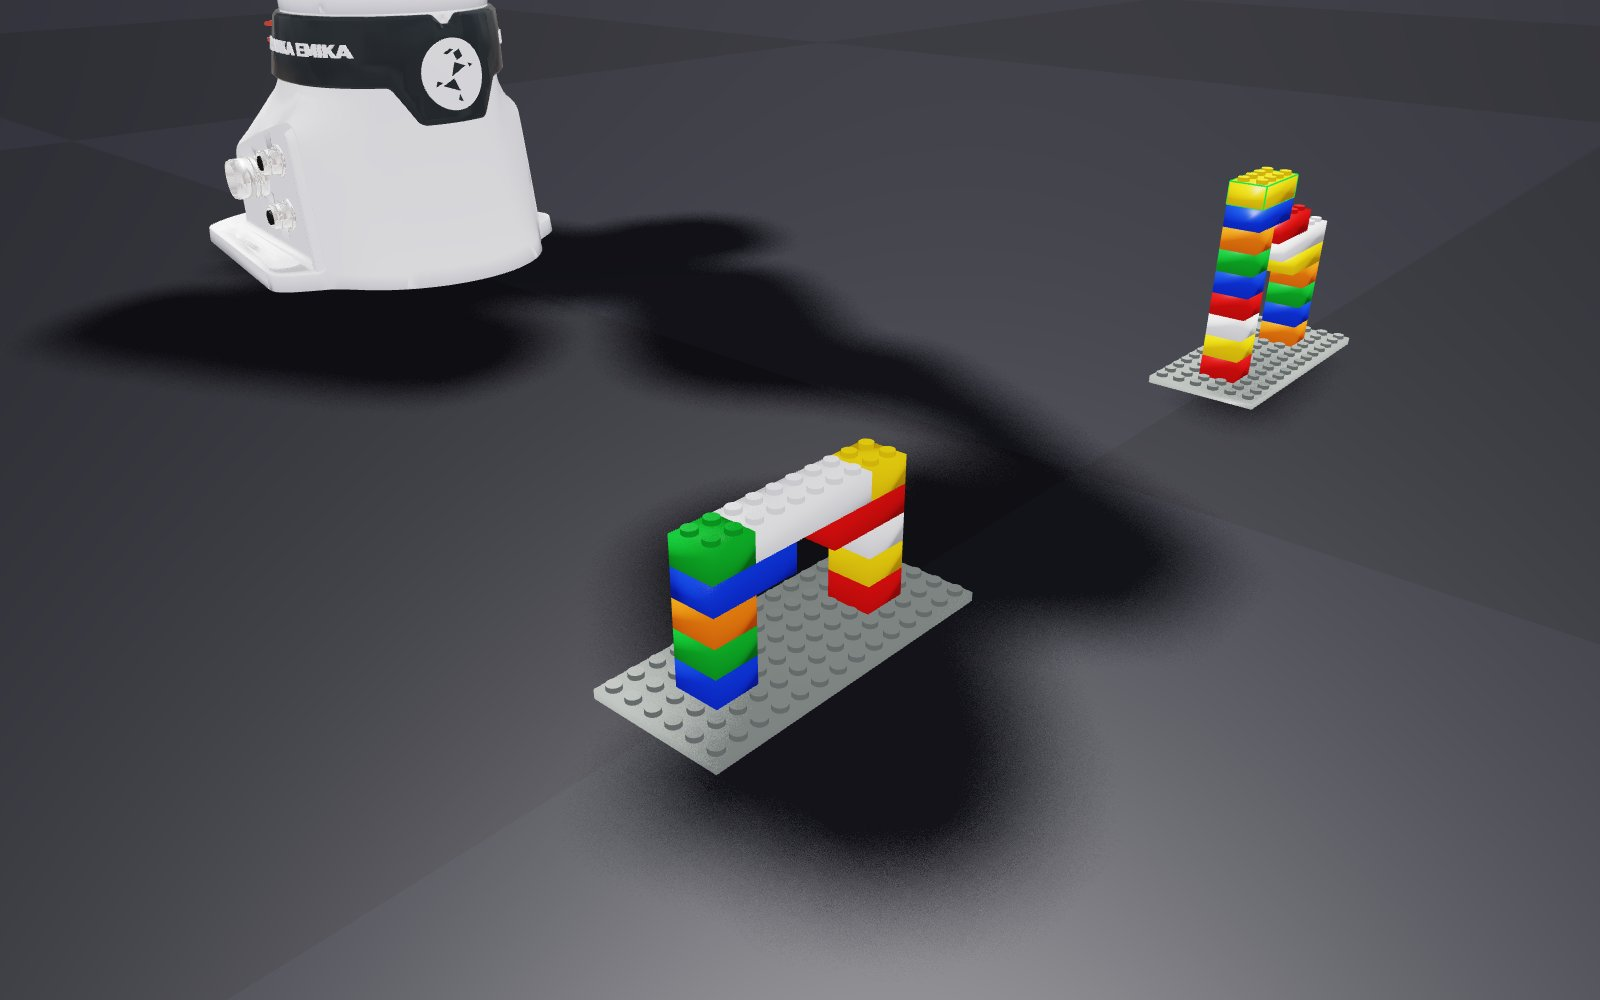
\includegraphics[width=\linewidth]{sim_a_fin_arch.jpg}\caption{Arch (front) and S3 (back).}\end{subfigure}\hfill
\begin{subfigure}{.49\linewidth}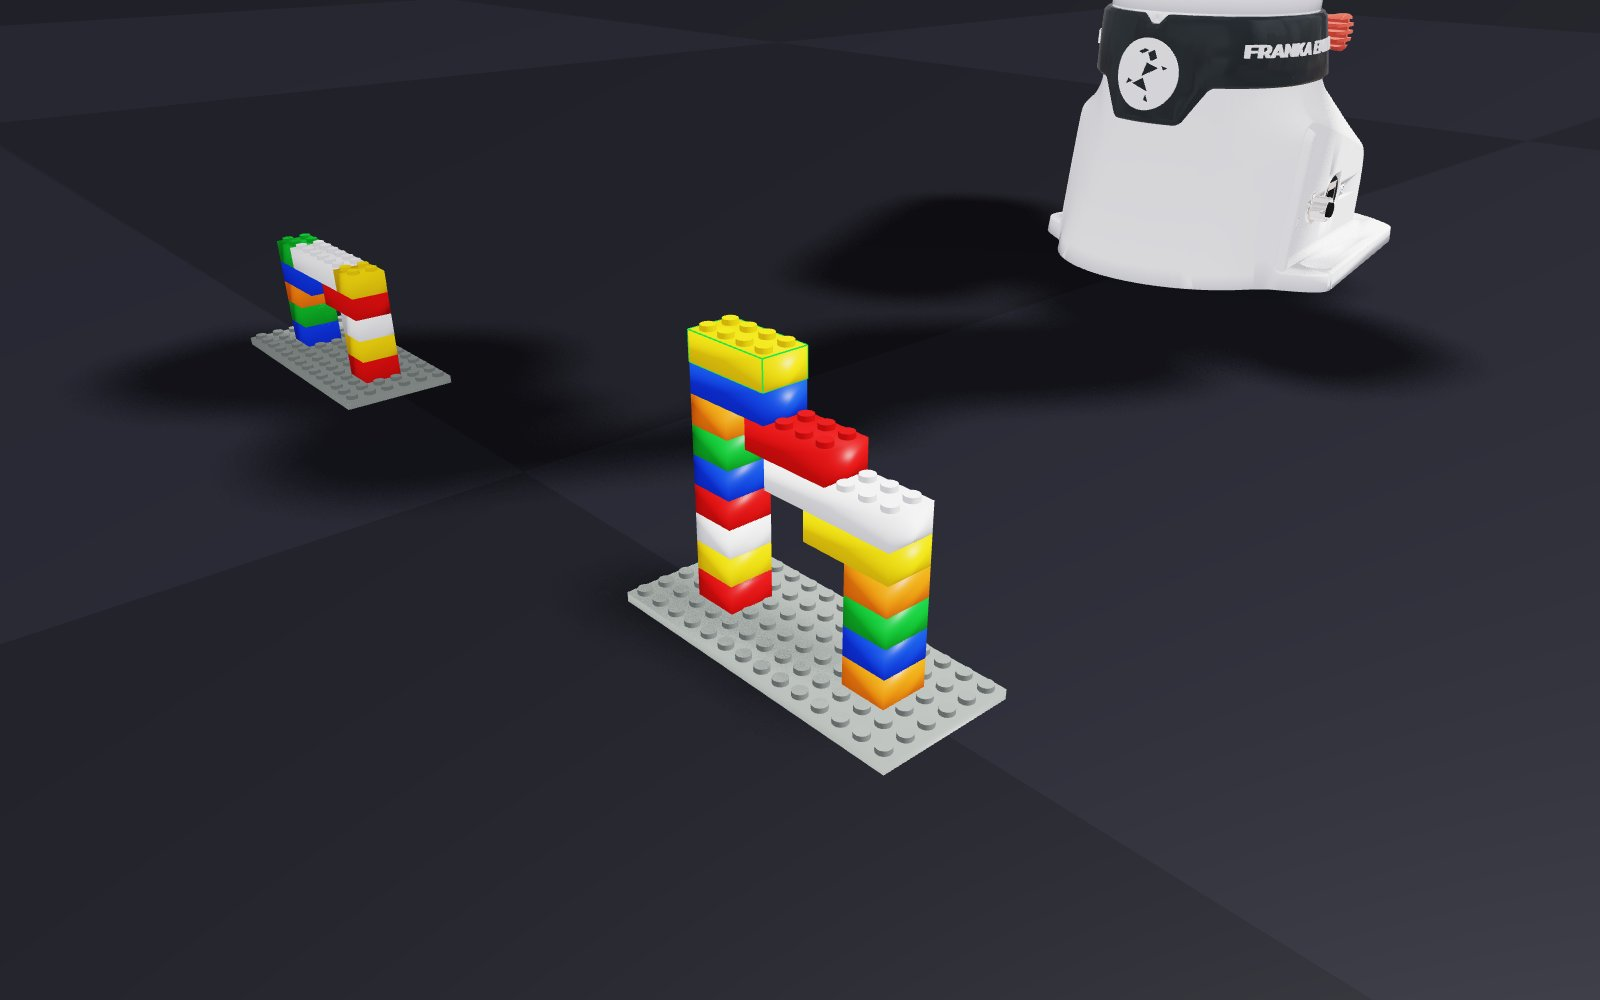
\includegraphics[width=\linewidth]{sim_a_fin_s3.jpg}\caption{S3 (front) and arch (back).}\end{subfigure}
\caption{The two finished structures at the end of the validated run. Each colour is one brick.}
\end{figure}

% =====================================================================
\section{The simulated work cell}\label{sec:cell}

Everything runs in a physics simulation; no physical robot was used.

\begin{itemize}
\item \textbf{Robots.} Two 7-joint Franka Research~3 arms with parallel-jaw
      grippers, facing each other 0.9\,m apart (arm A at $x=-0.45$\,m, arm B at
      $x=+0.45$\,m).
\item \textbf{Workspaces.} Each arm has its own studded build pad (0.32\,m apart,
      along $y$) and its own row of feeder bricks waiting on the table.
\item \textbf{Physics.} Newton 1.2.1 with the MuJoCo solver on the GPU, 60
      frames per second, 16 sub-steps per frame (about 1\,ms), implicit
      integration and elliptic friction cones. Newton's own collision pipeline is
      used because it keeps the small stud--wall contacts that other contact
      generators dropped.
\item \textbf{Bricks.} A brick has a visual mesh plus simple hidden collision
      shapes: a top slab, four walls and one cylinder per stud. Simple shapes are
      fast and give stable contacts.
\item \textbf{The ``click''.} Real studs grip by friction. In the simulation, once a
      brick passes the snap check (\S\ref{sec:done}) a set of \emph{weld}
      constraints switches on between it and each brick it sits on, one per stud
      patch. That is the clutch.
\item \textbf{Breaking.} Every frame the force carried by each weld is turned into
      a \emph{utilisation} $u$ with the same capacity law the planner uses
      (\S\ref{sec:support}). If $u\ge 1$ on two samples in a row, the weld is
      deleted, the brick is free, and the run fails. A plan that is too
      optimistic therefore shows up as a broken structure.
\end{itemize}

\begin{figure}[H]
\centering
\begin{subfigure}{.49\linewidth}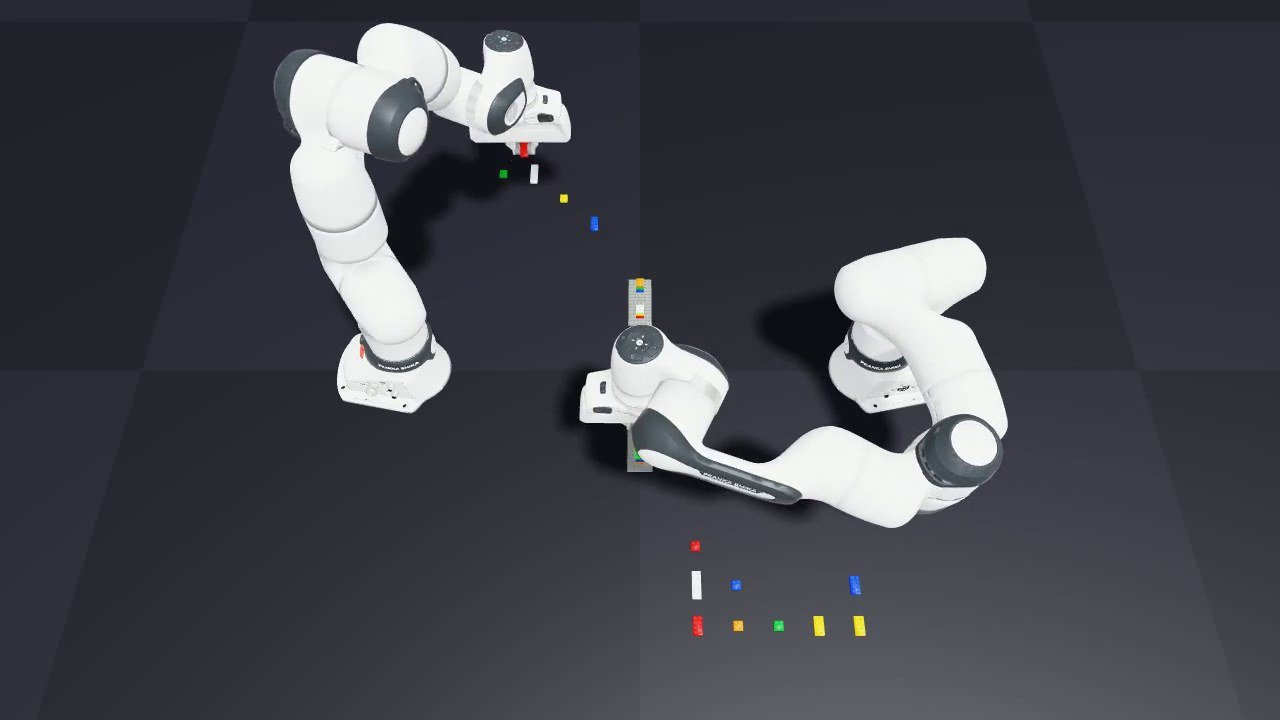
\includegraphics[width=\linewidth]{sim_overview_top.jpg}\caption{Overview: arm A (left) builds the arch, arm B (right) builds S3.}\end{subfigure}\hfill
\begin{subfigure}{.49\linewidth}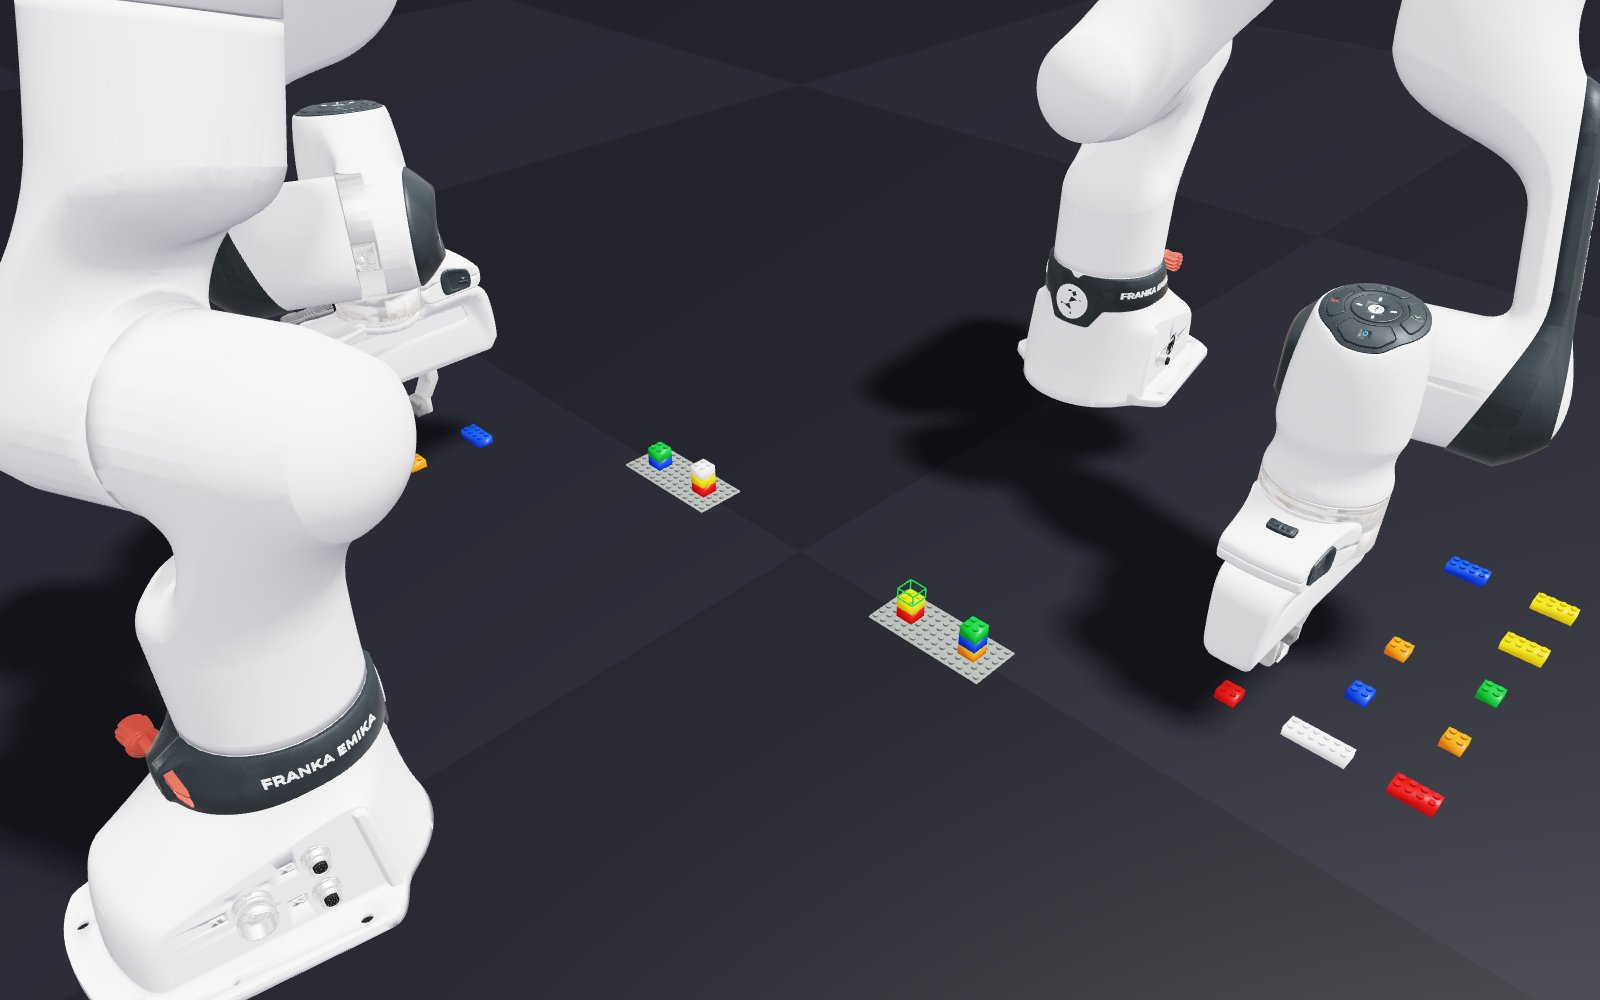
\includegraphics[width=\linewidth]{sim_a_over_120.jpg}\caption{Both arms working at the same time ($t=120$\,s); feeder bricks on the table.}\end{subfigure}
\caption{The simulated cell.}
\end{figure}

\why{The project needs contact-rich physics (fingers on bricks, bricks on studs)
for two arms at once, plus a way to break joints. Newton runs on the GPU,
exposes the per-constraint forces needed for the break rule, and integrates
with the same robot model that the motion planner uses. Welds are a
deliberate simplification: true stud interference is stiff and hard to
simulate, so the clutch is modelled by a snap check plus constraints. An
opt-in \texttt{--stud-fit} mode adds real insertion resistance
(\S\ref{sec:limits}).}

% =====================================================================
\section{Stage 1 -- Image to blueprint}\label{sec:blueprint}

\keyidea{Treat each drawing as a shadow of the model, carve a block of LEGO-sized
cubes until every shadow matches, then cover the remaining cubes with real
bricks, layer by layer, bonding them like a brick wall.}

\subsection{Inputs}

The input is one to three black-on-white silhouettes: a \emph{front} view
(columns are world $y$, rows are layers), and optionally a \emph{side} view
(columns are $x$) or a \emph{top} view. Polarity does not matter. Structures can
also be given directly as a brick list, which is how S3 is defined.

\begin{figure}[H]
\centering
\begin{subfigure}[b]{.3\linewidth}\centering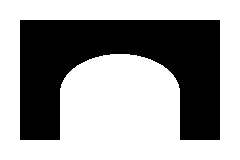
\includegraphics[width=.9\linewidth]{input_arch_front.png}\caption{Arch, front only (depth 2 studs).}\end{subfigure}\hfill
\begin{subfigure}[b]{.2\linewidth}\centering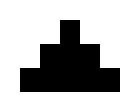
\includegraphics[width=.9\linewidth]{input_pyramid_front.png}\caption{Pyramid, front.}\end{subfigure}\hfill
\begin{subfigure}[b]{.2\linewidth}\centering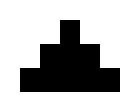
\includegraphics[width=.9\linewidth]{input_pyramid_side.png}\caption{Pyramid, side.}\end{subfigure}\hfill
\begin{subfigure}[b]{.24\linewidth}\centering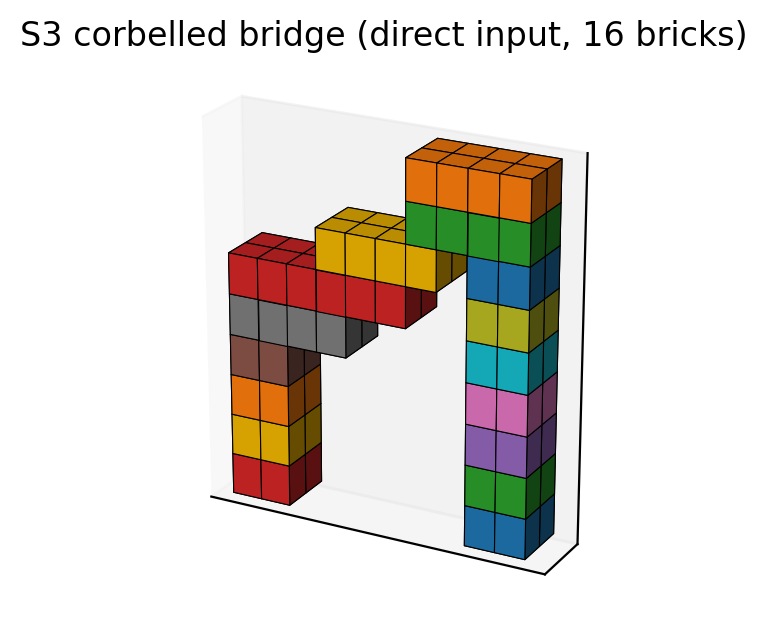
\includegraphics[width=.9\linewidth]{s3_bricks.png}\caption{S3, given as a brick list.}\end{subfigure}
\caption{The inputs used for the final runs. The pyramid was drawn by a user.}
\label{fig:inputs}
\end{figure}

\subsection{The algorithm, step by step}

\paragraph{1. Segment and crop.} The image is converted to grey. The threshold is
the midpoint between the darkest and brightest pixel. The average of the border
pixels tells which side is ``background'', so both dark-on-light and
light-on-dark drawings work. The mask is cropped to its bounding box.

\paragraph{2. Scale to the LEGO grid.} One stud is 8.0\,mm wide and one brick is
9.6\,mm tall. The user gives the width in studs (for example 5 for the
pyramid). The number of layers follows from the drawing's aspect ratio:
\[
\text{layers} = \operatorname{round}\!\Big(\text{width}\cdot\frac{\text{image height}}{\text{image width}}\cdot\frac{8.0}{9.6}\Big).
\]
The depth comes from the side or top view in the same way (default 2 studs).

\paragraph{3. Resample by majority vote.} The cropped mask is split into a grid of
(layers $\times$ studs) cells. A cell is \emph{full} if more than half of its pixels
are inside the shape. This removes drawing noise and slightly wobbly edges.

\paragraph{4. Carve the visual hull.} Start with a solid block $V[i,j,k]$ and keep a
cell only if every view sees it:
\[
V[i,j,k] = F[k,j] \wedge S[k,i] \wedge T[i,j].
\]
A missing view counts as ``all full''. This is the classic shape-from-silhouette
\emph{visual hull}.

\paragraph{5. Tile each layer with bricks (greedy, bottom-up).} The library is
2$\times$6, 2$\times$4, 2$\times$3, 2$\times$2, 1$\times$6, 1$\times$4,
1$\times$2, 1$\times$1, in both orientations. For each layer:
\begin{itemize}
\item Uncovered cells that have \emph{nothing underneath} (overhangs) are handled
      first. Tying them in early is what joins the two legs of the arch.
\item For an anchor cell, every brick placement that covers it without overlap
      is scored, and the best one is kept. The score is compared in this order:
      \begin{enumerate}[nosep]
      \item rests on the \textbf{most different bricks below} (ties structures together);
      \item creates the \textbf{fewest seams on top of seams} (running bond, like a wall);
      \item \textbf{bigger} bricks;
      \item long axis \textbf{alternates} between layers (cross-bonding);
      \item closer to the layer's centre.
      \end{enumerate}
\item A brick above layer 0 must sit on at least one brick. If no placement can
      reach a cell, the shape overhangs too far and the program stops with that
      message instead of producing something unbuildable.
\end{itemize}

\paragraph{6. Number the bricks} in the order the planner will build them (\S\ref{sec:plan}).

\begin{figure}[H]
\centering
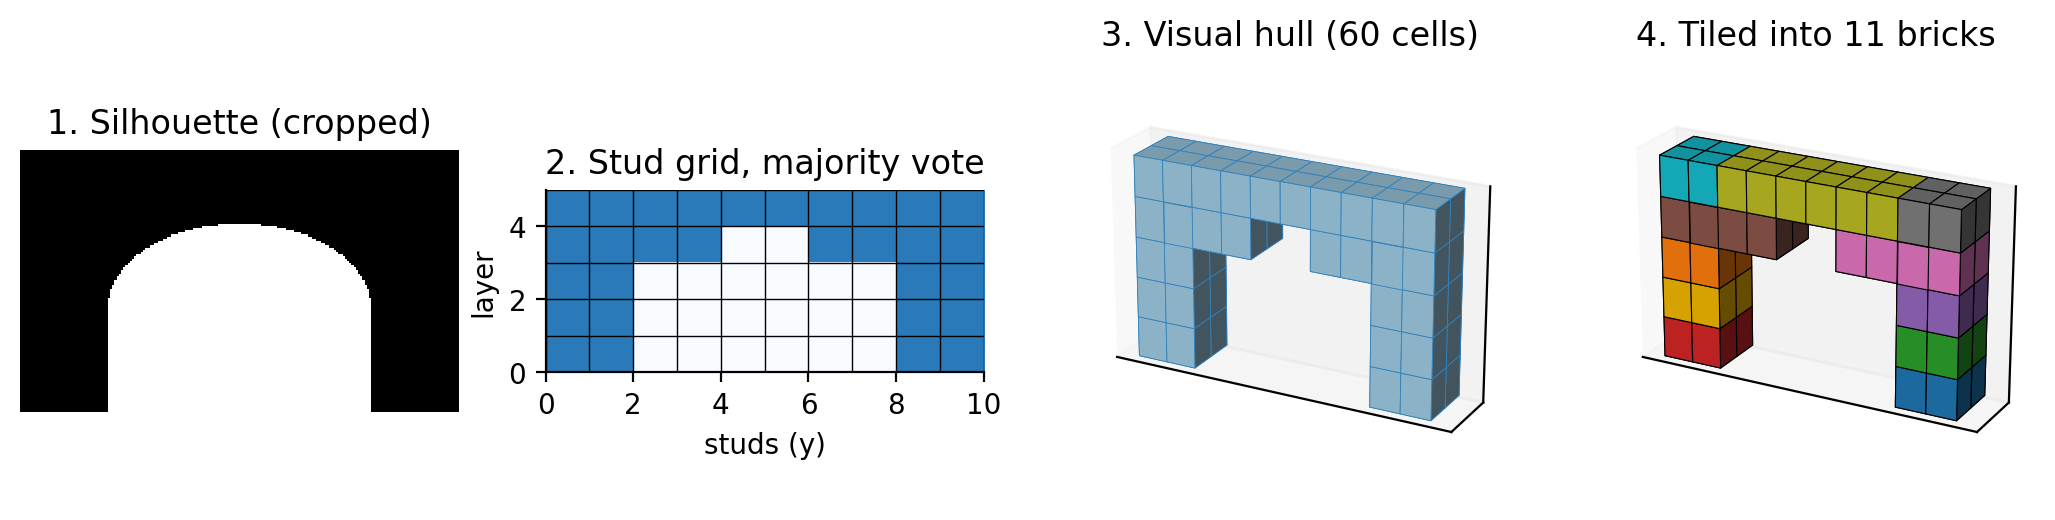
\includegraphics[width=\linewidth]{pipeline_arch.png}\\[2mm]
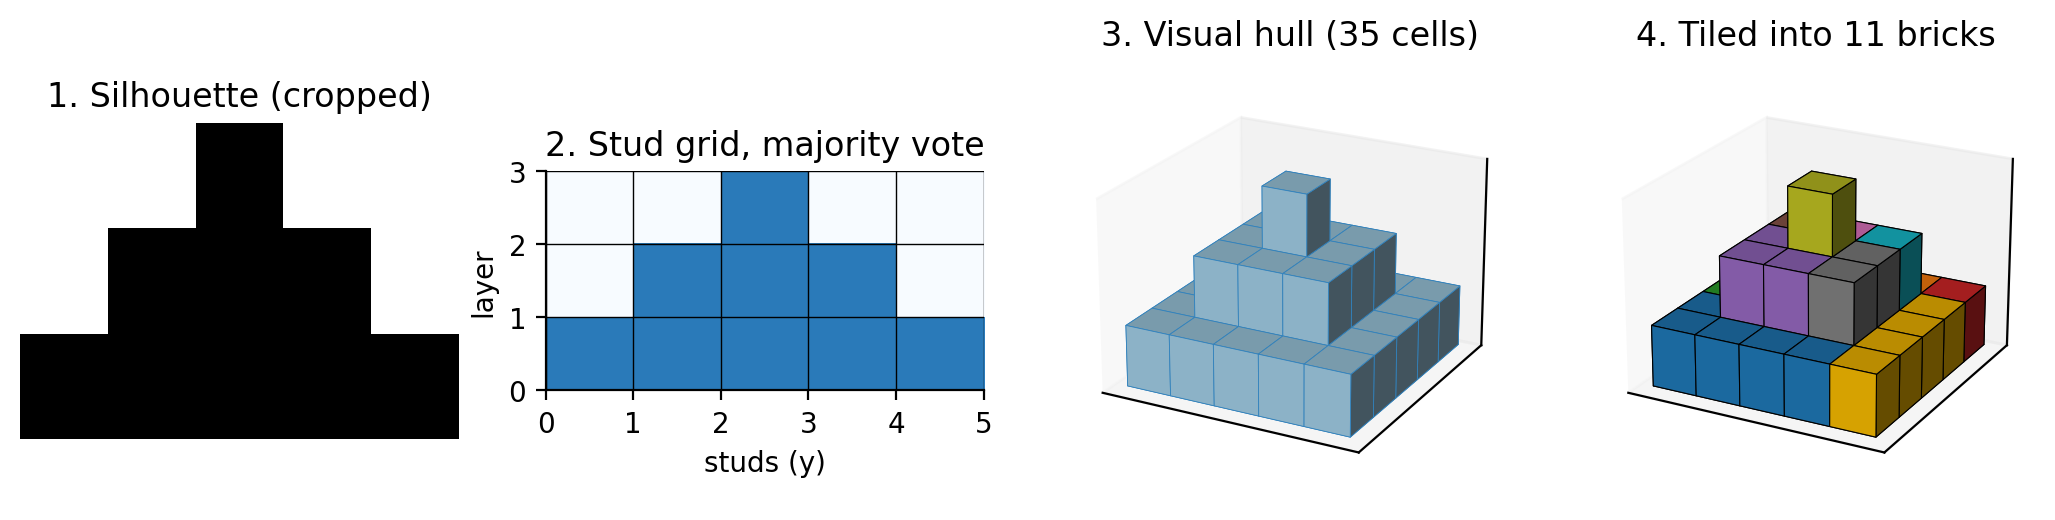
\includegraphics[width=\linewidth]{pipeline_pyramid.png}
\caption{Image to blueprint for the arch (top) and the user's pyramid (bottom):
the drawing, the majority-vote grid, the carved visual hull, and the tiled
bricks (one colour per brick). The round arch becomes a stepped (corbelled)
arch on the grid, which is exactly the overhanging case that needs a helper arm.}
\label{fig:bp}
\end{figure}

\begin{figure}[H]
\centering
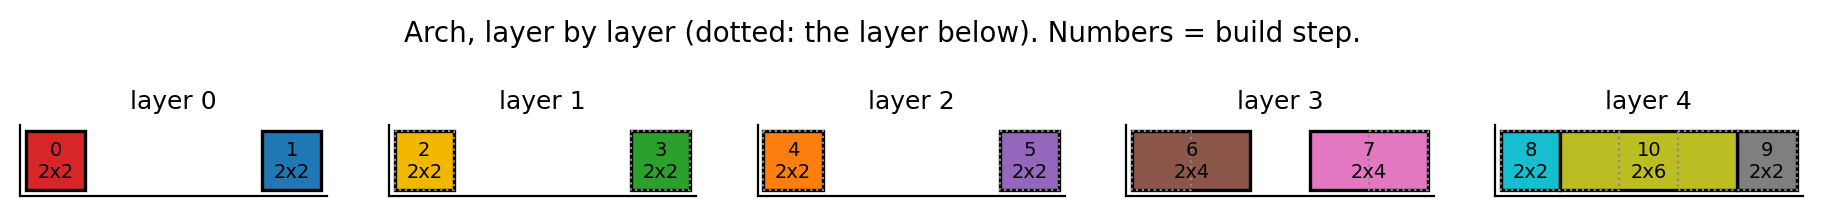
\includegraphics[width=\linewidth]{layers_arch.png}\\[1mm]
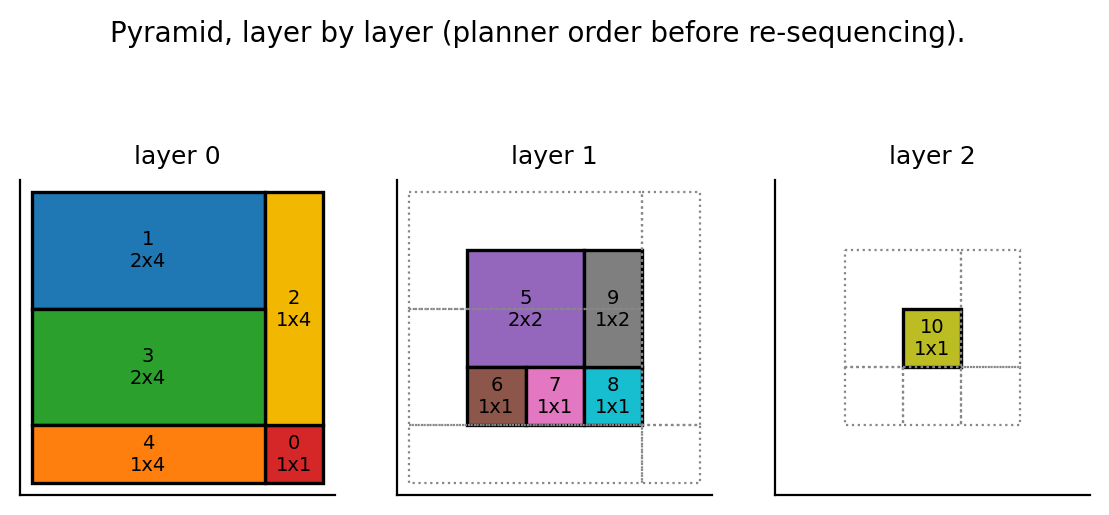
\includegraphics[width=.55\linewidth]{layers_pyramid.png}
\caption{The tiling, layer by layer, seen from above. Numbers are build steps.
In the arch, layers alternate long axes, and the 2$\times$6 crown (step 10)
spans the gap and rests on both legs.}
\end{figure}

\why{Silhouette carving needs no learning, no training data and no camera
calibration, and it is exact for the shapes LEGO is good at (extrusions,
arches, walls, stepped pyramids). Its known limit is that it cannot see a
hidden hollow, which it fills in; a single photo of an arbitrary object would
need an image-to-3D model first. Greedy tiling with a lexicographic score is
fast (milliseconds), predictable and easy to explain. Each criterion encodes
a rule a human builder follows: tie parts together, stagger seams, prefer big
bricks, cross the layers. A global search (beam search) was not needed for
these shapes.}

% =====================================================================
\section{Stage 2 -- Blueprint to plan}\label{sec:plan}

\keyidea{For every brick, the plan states when it goes on, exactly where, how the
gripper should hold it, where to press it, and whether the other arm must hold
the structure meanwhile.}

\subsection{Build order}
Bricks are sorted bottom layer first. A brick may only be placed after every
brick under it, and a brick with nothing below raises an error (``floating'').
Inside a layer, square 2$\times$2 bricks go first. Their faces are only 16\,mm
long while a fingertip pad is 17.5\,mm wide, so a 2$\times$2 gripped next to an
in-line neighbour would rub that neighbour; placed first, it has none.

A second rule handles boxed-in small bricks (\texttt{small\_first} in
\texttt{dual\_build.py}). If a layer contains a 1$\times$1 that the fingers cannot
reach once its neighbours are in, that layer is re-ordered \emph{fewest studs
first}. A 1$\times$1 sits on a single stud, so it cannot simply be dropped (it
tips over); it has to be held all the way down while there is still room for
the fingers. All other layers keep the normal order.

\subsection{Target pose}
Each brick's grid position $(i,j,k)$ and orientation give its world pose. The
plan also stores a \emph{pre-insertion} pose 25\,mm straight above the target,
where the arm switches from free-space motion to a slow straight descent.

\subsection{Grip choice}
The gripper squeezes two opposite faces. The planner counts, for each pair of
faces, how many already-placed bricks in the same layer the 17.5\,mm pads would
touch, and picks the pair that touches fewest (short side on a tie). The grip
width is the brick width minus 1.2\,mm.

\subsection{Press point}
If a brick only partly rests on bricks below (an overhang), pressing its centre
can tip it or pry a joint open. The planner slides the grip along the brick,
keeping the pads on it, and evaluates the force model of \S\ref{sec:support} at
2\,mm steps. It keeps the offset with the lowest predicted joint load
(\texttt{best\_press\_point}).

\why{A layer-by-layer greedy order is always physically valid (nothing is placed
in mid-air) and is easy to check. A smarter per-layer search for an order with
no finger contact was tried and reverted: on the arch it pushed the crown last,
into a slot with 0.1\,mm to spare at each end, which was worse. Grip and press
choices are made with simple, explainable rules and the same force model as the
support check, so the plan and the support decision agree.}

% =====================================================================
\section{Stage 2b -- Stability check and temporary support}\label{sec:support}

\keyidea{Before every step, imagine the press, compute how close each stud joint is
to popping off with a linear program, and if any joint is too close, choose the
place where the other arm's grip helps that joint most.}

\subsection{How a stud joint fails}
A LEGO joint can be pushed together almost without limit (the brick rests on
the one below), but can only be pulled apart up to the friction of its studs:
about 11.3\,N per stud. Pushing a brick on needs about 8.9\,N per stud. When an
arm presses a brick onto the far end of an overhang, the push acts like a
person standing at the end of a diving board: it levers the joint at the root
open.

\subsection{Capacity of one joint}
Take the overlap patch between an upper brick and the brick below. Compression
may act anywhere in the patch, tension only at the studs, at most $f_b=11.3$\,N
each. For a load given by an axial force $F_z$ and two moments $M_x, M_y$, the
utilisation $u$ (the fraction of the joint's capacity in use) has a closed form,
one term per patch edge $e$:
\[
u = \max\Big(0,\ \max_{e}\ \frac{(\mathbf n_e\!\cdot\!\mathbf q_e)F_z - n_{e,y}M_x + n_{e,x}M_y}{f_b\,D_e}\Big),
\]
where $\mathbf n_e$ is the inward normal of edge $e$, $\mathbf q_e$ a point on it,
and $D_e$ the summed lever arms of the studs about that edge. In words:
\emph{the prying moment about an edge divided by the most moment the studs can
resist about that edge}. $u<1$ holds; $u\ge 1$ breaks.

\subsection{Force balance of the whole partial structure}
For the bricks already placed, the planner writes force and moment balance for
every brick (gravity, the insertion press, and any support) and lets the joint
forces be unknowns. A \textbf{linear program} (SciPy \texttt{linprog}) finds the
distribution that \emph{minimises the largest utilisation} $s$ over all joints:
\begin{align*}
\min\ & s\\
\text{s.t. } & \text{force and moment equilibrium of every brick},\\
& u_c \le s \quad\text{for every joint } c,\\
& \text{support forces within the grip's friction and force limits}.
\end{align*}
By the lower-bound theorem of plastic analysis, if $s<1$ some admissible set of
forces exists and the structure holds. The press is $n_\text{studs}\times 8.9$\,N
at the mating studs, and the analysis is repeated with a 3\,N sideways
disturbance in four directions; the worst case is kept. This model agreed with
the independent BrickSim static solver on S3 (both give $u=2.36$ for the same
test press).

\subsection{When is support needed, and where?}
\begin{enumerate}
\item \textbf{Trigger.} A step needs support if $u \times 3 \ge 1$ (a safety factor of 3).
      The factor was set from a measured gap: the simulated joints are brittle and
      compliant (a tall pier leans and adds load), which a rigid-plastic model
      underestimates.
\item \textbf{Weakest joint.} The joints whose $u\times 3\ge 1$ are the problem
      joints; their bricks are the targets.
\item \textbf{Candidate grips.} Every stud column along the structure, at every
      seam and quarter height. A candidate is kept only if the 17\,mm pads are
      above the baseplate studs, mostly backed by bricks, and far enough from the
      placing hand (the helper leans its hand 45$^\circ$ away).
\item \textbf{Score.} Each candidate is added to the LP as a bounded grip (friction
      $\mu\cdot 2\cdot 14.3$\,N shared among the gripped bricks by contact area, a
      moment limit, and the arm's force limit). The grip with the lowest predicted
      utilisation wins; ties are broken at the 1.3$\times$ press the robot really
      applies, then by the least-loaded grip.
\item If no grip is feasible, planning stops with ``no feasible support''.
\end{enumerate}

\begin{figure}[H]
\centering
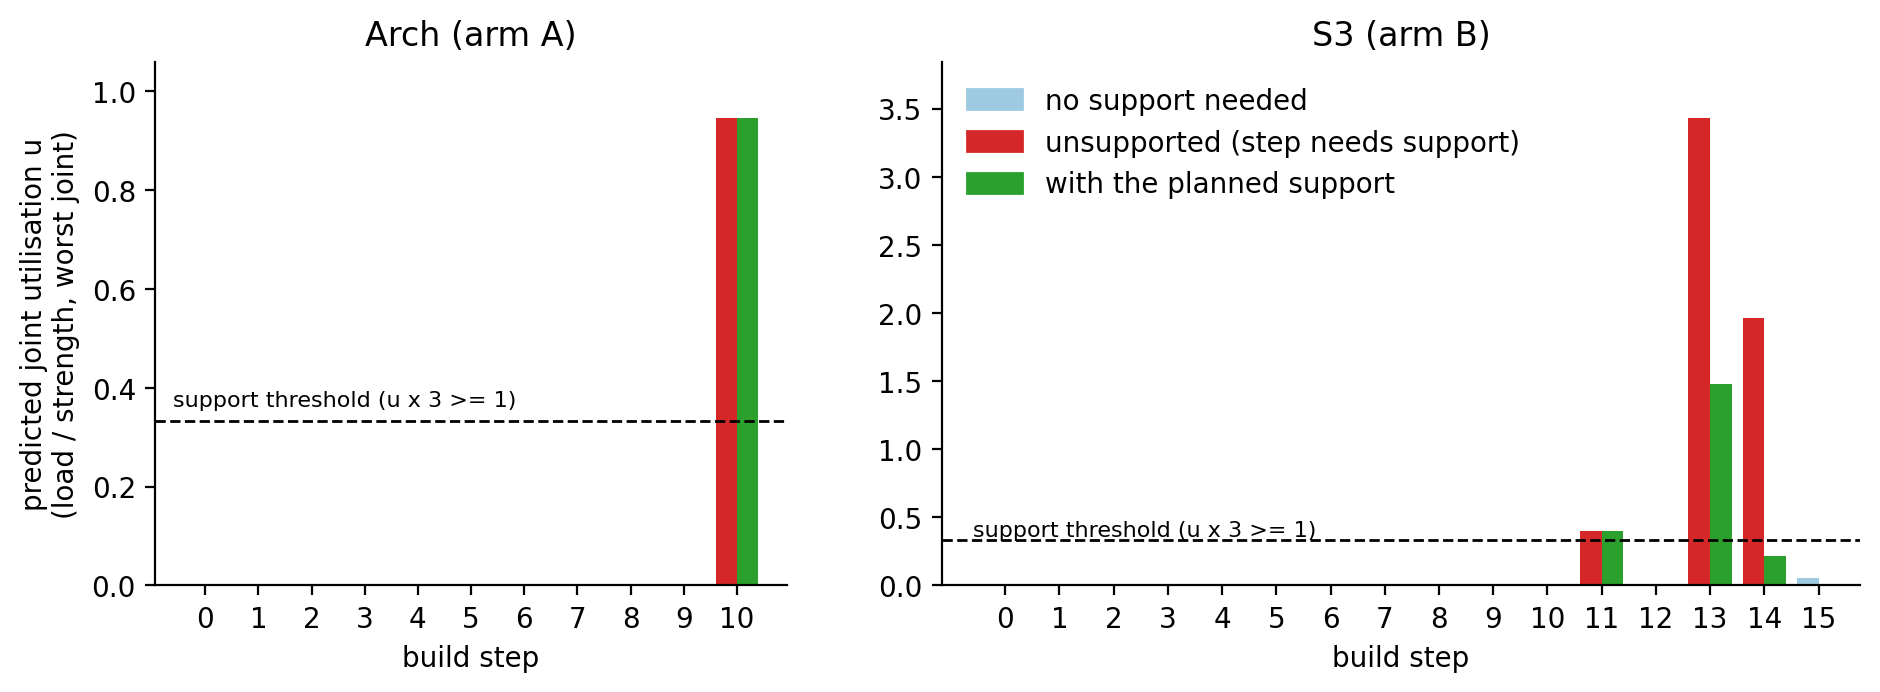
\includegraphics[width=\linewidth]{utilisation.png}
\caption{Predicted worst-joint utilisation at every step, read from the saved
plans. Red: steps over the support threshold, which become supported steps. Green:
the same step with the planned support. The arch needs support only for its
crown (step 10); S3 needs it at steps 11, 13 and 14.}
\label{fig:util}
\end{figure}

\begin{figure}[H]
\centering
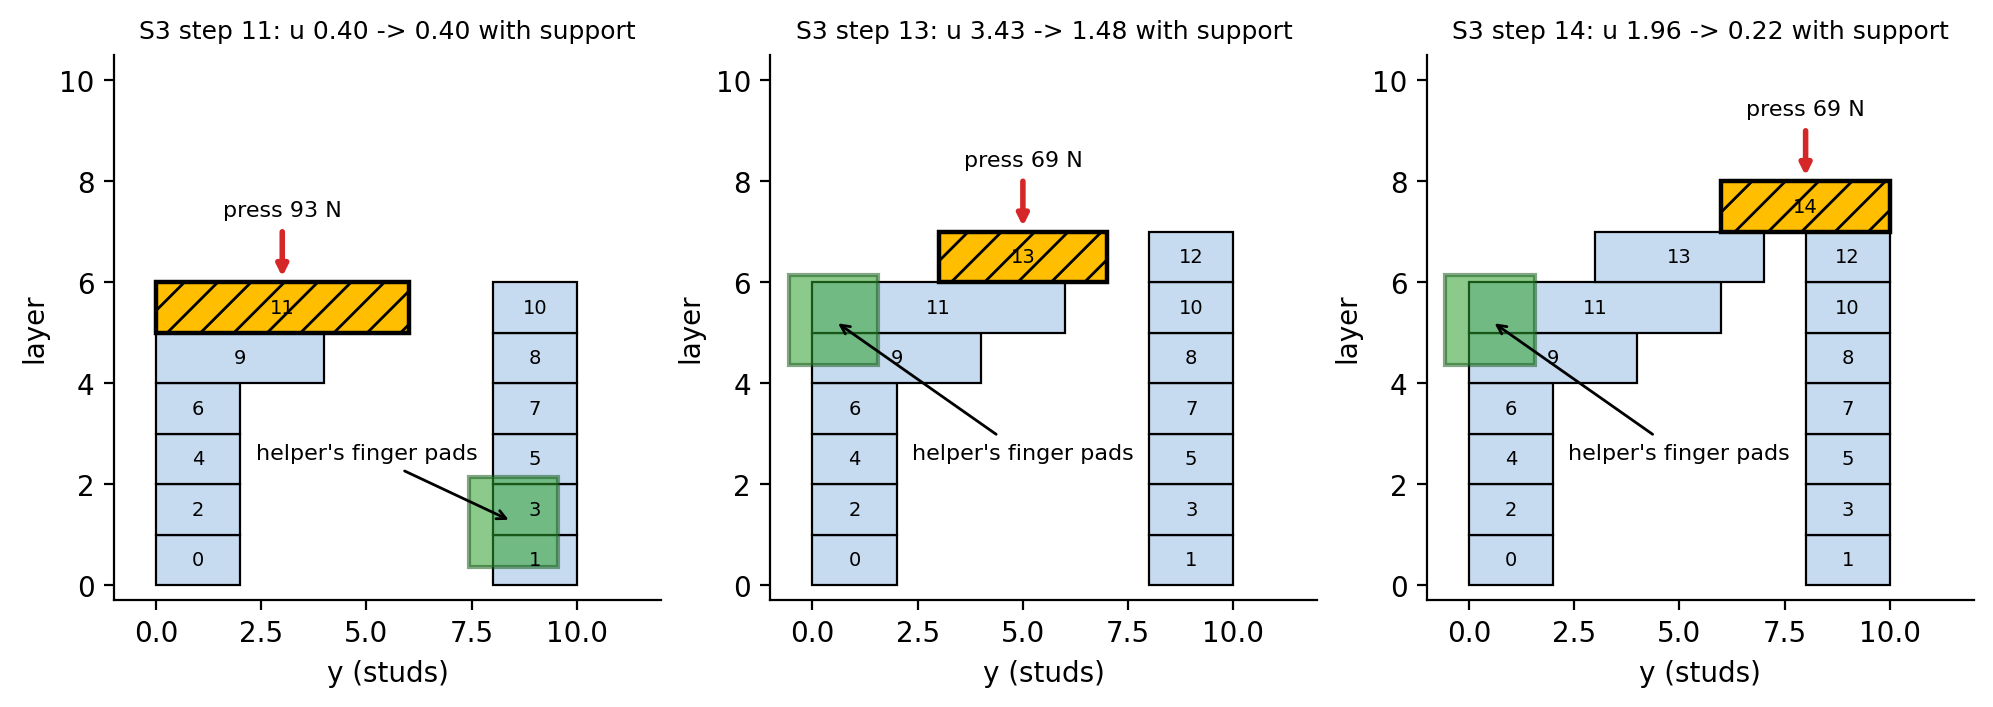
\includegraphics[width=\linewidth]{s3_supports.png}
\caption{S3 seen from the side at its three supported steps: the brick being
pressed (hatched), the press, and where the helper's finger pads close. At
step 13 the corbel being pressed overhangs the left pier; a grip at the pier
top cuts the predicted load from 3.43 to 1.48.}
\label{fig:s3sup}
\end{figure}

\why{The project's main contribution is deciding \emph{where} a second arm should
hold. A nearest-brick heuristic ignores how load travels; a learned policy
needs data we do not have. The force-balance LP is the established method for
LEGO stability (StableLego), it is fast (milliseconds per step), it includes
the helper's grip directly as extra bounded forces, and it can be checked
against an independent solver. Because the simulator breaks joints with the
\emph{same} capacity law, planning and execution use one definition of
``too much load''.}

\paragraph{Honest reading of Figure~\ref{fig:util}.} For S3 steps 13 and 14 the
planned grip lowers the predicted load a lot. For the arch crown and S3 step 11
the best reachable grip does not lower the model's number, because the critical
joint is at the base of a pier, which the helper cannot grip without colliding
with the plate or the placing hand. These supports are still executed. The
model is conservative: in the default simulation the press needed is smaller
than the 8.9\,N-per-stud design press, and no joint broke in any validated run.

% =====================================================================
\section{Stage 3 -- Plan to control}\label{sec:control}

\keyidea{Each plan step becomes a short list of named moves; long moves are planned
by a GPU motion planner around every obstacle, the last few centimetres are
straight lines, and an inverse-kinematics solver turns hand targets into joint
angles 60 times a second.}

\subsection{Moves as a waypoint queue}
For each brick, the plan step becomes a queue of moves (``phases''):

\begin{center}
\small
\begin{tabular}{@{}lll@{}}
\toprule
Phase & What happens & How it is driven \\
\midrule
to feeder & travel high to above the brick & planned (cuRobo) \\
descend, settle, grasp & go down, wait for the arm to catch up, close & straight line \\
lift & rise with the brick & straight line \\
transport & carry above everything to the pre-insert point & planned (cuRobo) \\
pre-insert, insert & slow descent onto the studs, brick-aim servo active & straight line \\
(wriggle / press) & only for tight slots or drop-and-press & straight line \\
release, retract & open while rising 2\,mm, lift away & straight line \\
clearance / park & return to a checked safe pose & planned (cuRobo) \\
\bottomrule
\end{tabular}
\end{center}

Each move is eased with a \emph{smoothstep} profile $s=3x^2-2x^3$ (zero speed at
both ends). A move ends when its time is up, the hand has arrived within 3\,mm,
and any condition it waits for (for example ``the helper is holding'') is true.
A wait longer than 30\,s is reported as a deadlock.

\subsection{Free-space motion: cuRobo}
For the long moves, the controller asks NVIDIA \textbf{cuRobo} for a joint
trajectory from the arm's measured joints to the goal. cuRobo represents the
arm as a chain of spheres and the world as boxes (both build pads and
structures, all feeder bricks, the table, and the other arm), and solves a
GPU-parallel trajectory optimisation from many seeds that minimises a cost
including collision distance, smoothness and joint limits. The brick in the
hand is attached to the arm as 12 inscribed spheres so it is avoided too. The
trajectory is played back at half speed.

\subsection{The last 30 millimetres: straight lines}
Close to contact, a planner that avoids every obstacle cannot work: the goal
\emph{is} contact. So the final 30\,mm of every approach is a straight
Cartesian line, sampled every 2\,mm and checked (\S\ref{sec:collision}).

\subsection{Hand target to joint angles: inverse kinematics}
Every frame, the hand target of each arm is converted to joint angles by
Newton's IK solver: a damped least-squares (Levenberg--Marquardt) solver with an
analytic Jacobian, objectives for hand position, hand orientation and joint
limits, 24 iterations per frame, both arms solved together as one batch. The
joint angles are sent to stiff joint position controllers (400\,N\,m/rad).

\subsection{Aiming the brick, not the hand}
A brick can slip slightly in the fingers, and the studs only allow 0.6\,mm of
play per side. So during the descent the controller measures where the
\emph{brick} is and nudges the hand target with an integral servo (gain 4\,s$^{-1}$,
limited to $\pm$4\,mm) until the brick's centre is over its target. The servo is
paused while the scheduler holds that arm still; otherwise its integral would
``wind up'' and later push the brick off target (this exact bug caused a miss
in run 011 and was fixed).

\begin{figure}[H]
\centering
\begin{subfigure}{.32\linewidth}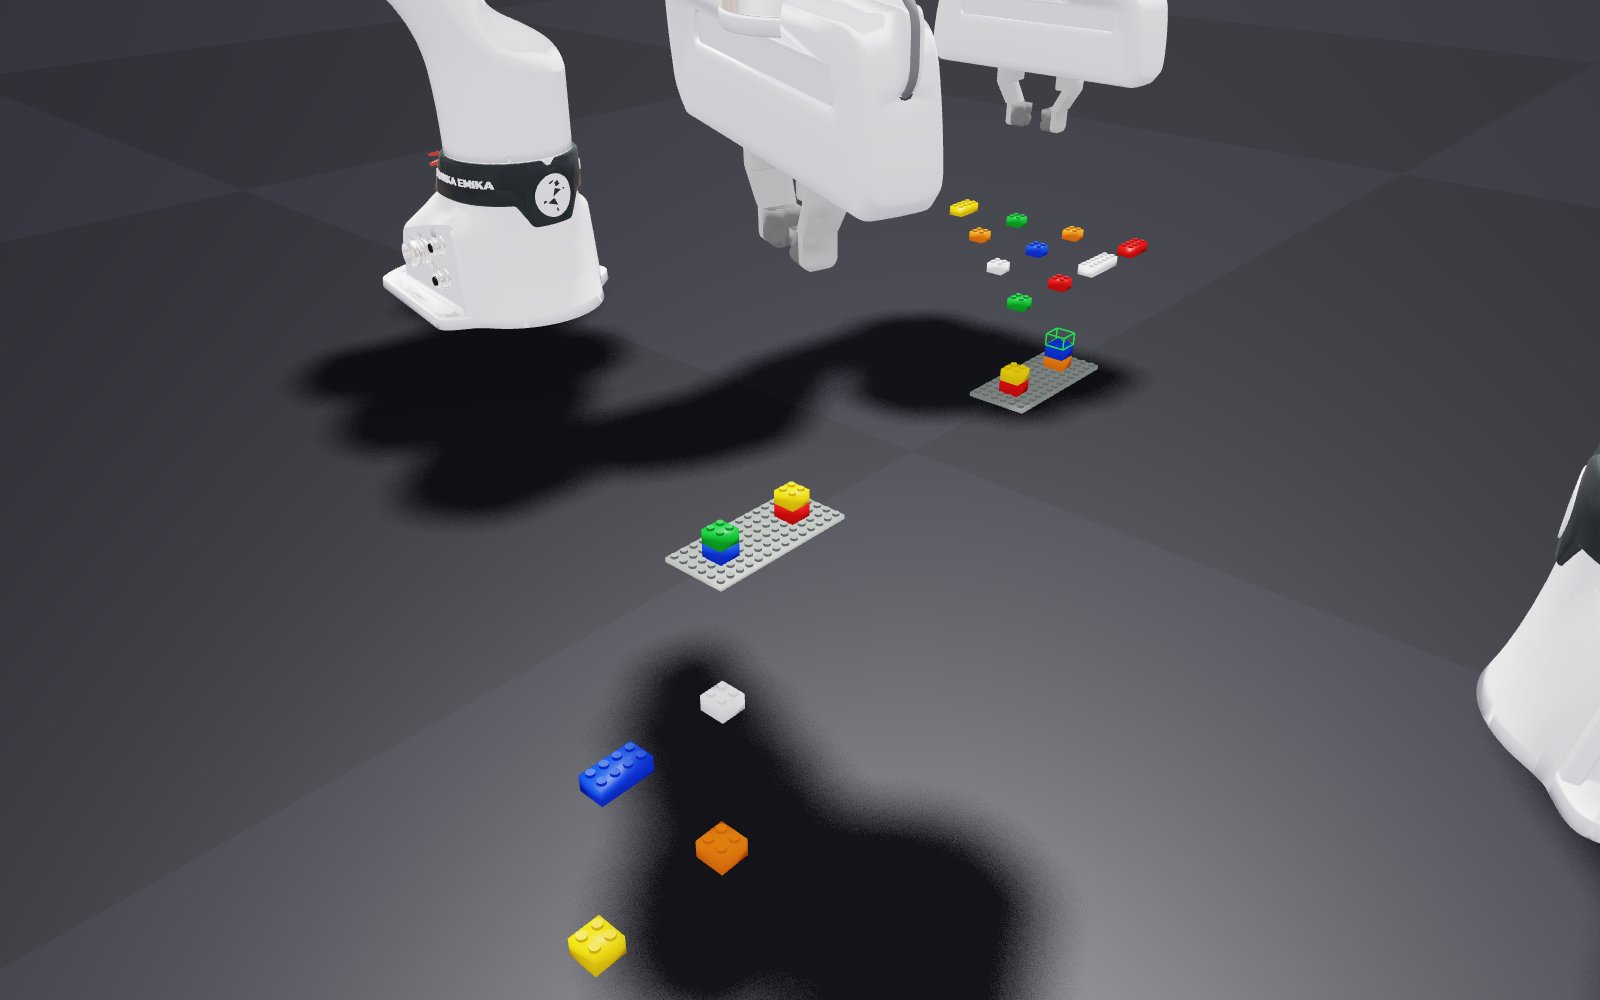
\includegraphics[width=\linewidth]{sim_a4_090.jpg}\caption{Over the feeder.}\end{subfigure}\hfill
\begin{subfigure}{.32\linewidth}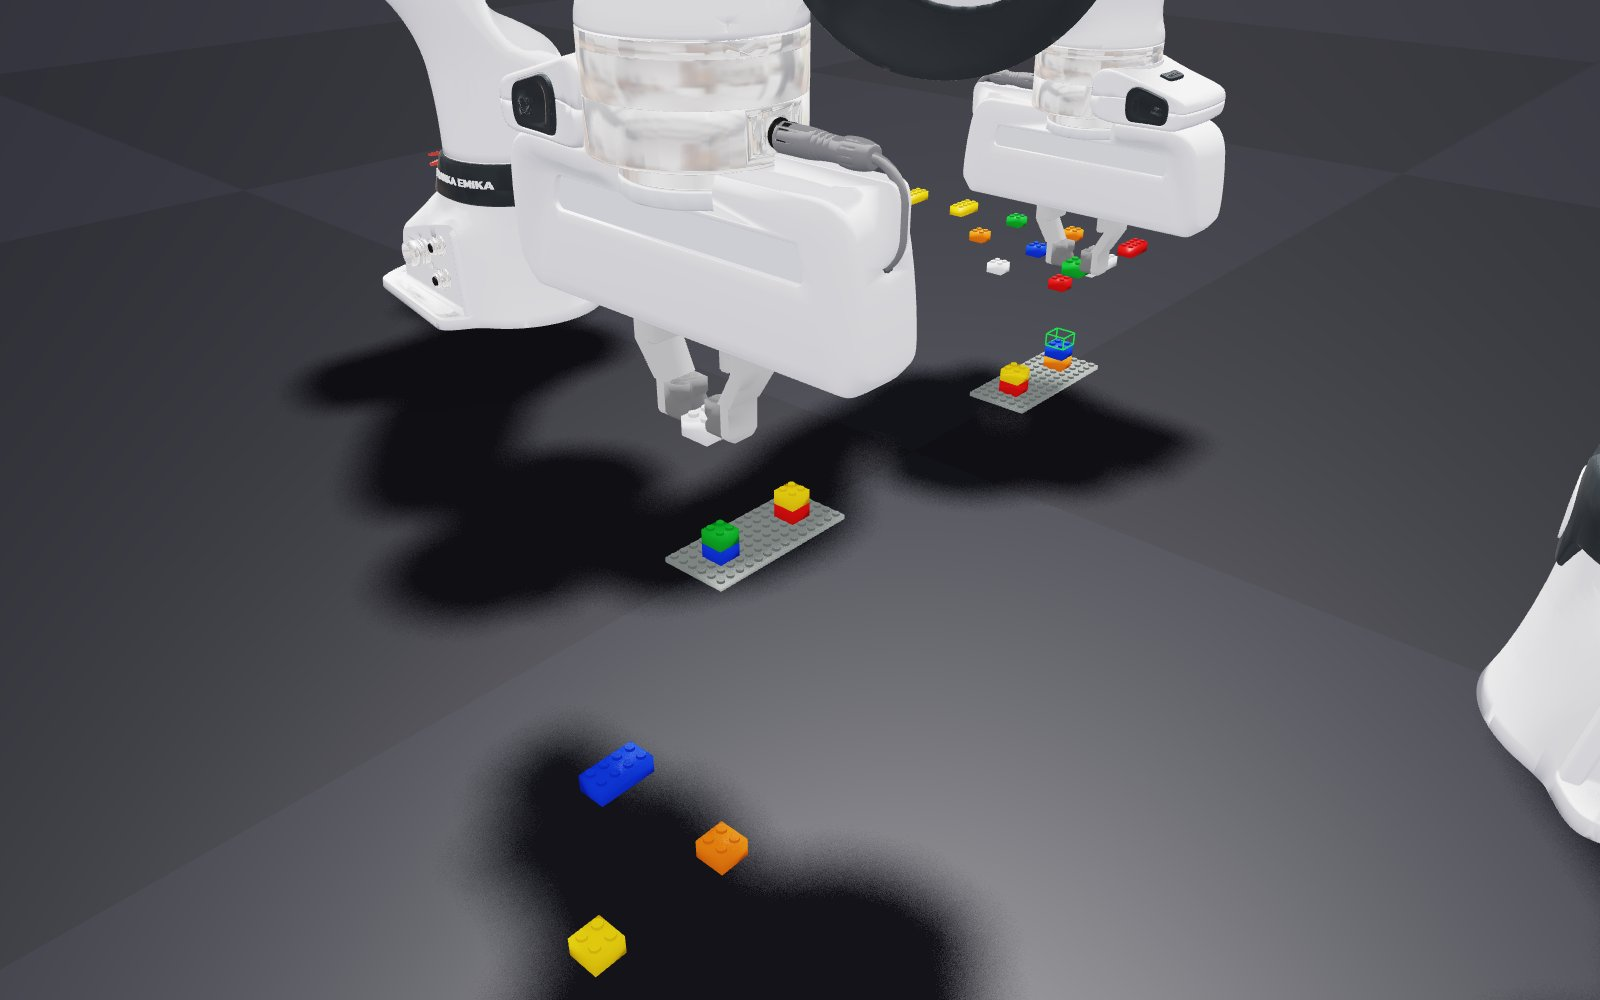
\includegraphics[width=\linewidth]{sim_a4_098.jpg}\caption{Transport (planned path).}\end{subfigure}\hfill
\begin{subfigure}{.32\linewidth}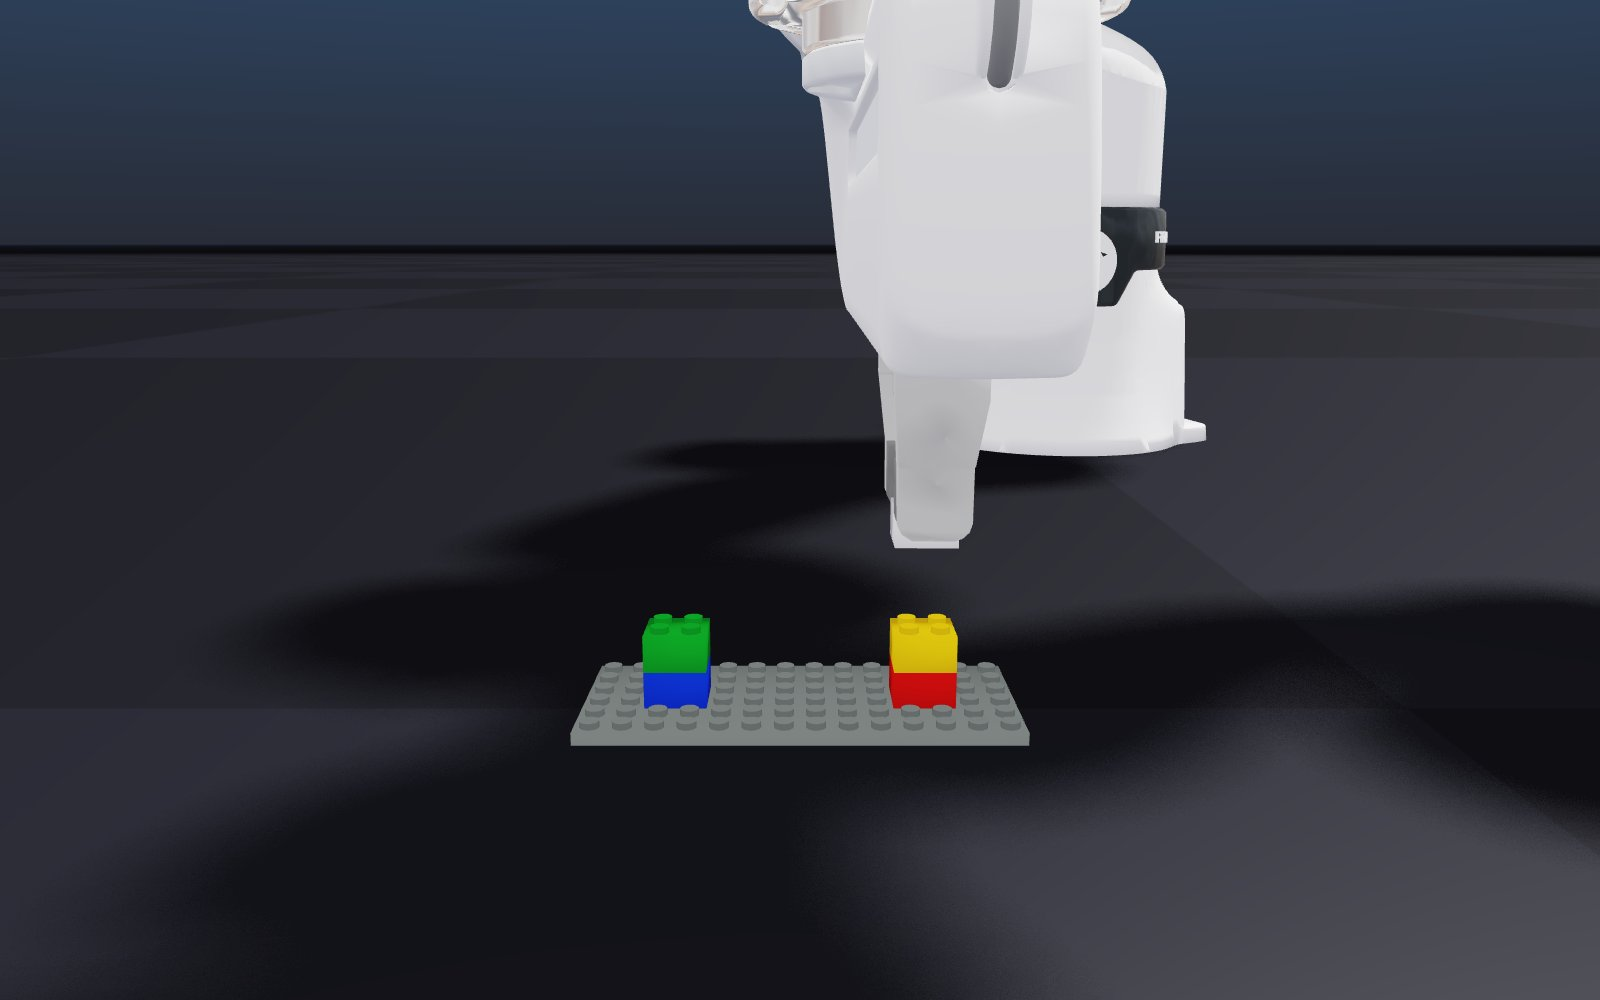
\includegraphics[width=\linewidth]{sim_a4_104.jpg}\caption{Straight insertion.}\end{subfigure}
\caption{One pick-and-place (arch step 4) in the validated run.}
\end{figure}

\why{Splitting control into ``plan the big moves, script the small ones'' uses
each tool where it is strong. cuRobo plans a collision-free 7-joint path in
tens of milliseconds on the GPU with an exact robot model; a hand-written
planner would be slower and less safe. Straight lines are the only sensible
motion for contact, and are easy to check densely. Damped least-squares IK is
robust near singular poses and runs batched on the GPU. The brick-aim servo
closes the loop on the quantity that matters (the brick's position) with a
single tunable gain.}

% =====================================================================
\section{Manipulation}\label{sec:manip}

\keyidea{The builder picks the grip that physically fits, inserts with the brick
aimed over the studs, wiggles into tight slots, and drops-and-presses when no
side grip fits; the helper approaches carefully, grips firmly, and stays still
while the builder works.}

\subsection{Grip selection with fallbacks}
Before each pick, the controller checks the full finger-sphere model at the
\emph{seat} of the brick, with the fingers open and closed, against everything
around it (\texttt{pickup\_clearance}). It tries, in order, and keeps the first
that clears by 1.5\,mm:
\begin{enumerate}[nosep]
\item the planner's grip;
\item the other pair of faces, centred;
\item edge grips, nearest first, keeping at least 70\% of the face under the pad;
\item otherwise \textbf{drop-and-press}.
\end{enumerate}
A grip may also rise by up to 2\,mm so the fingertips clear the studs of the
layer below.

\subsection{Drop-and-press}
When the fingers cannot reach down beside a brick (flush neighbours on both
sides), the arm lowers the brick only until open and closed fingers clear the
neighbours by 1.5\,mm, waits, releases, rises, closes its fingers into a
``fist'', and presses the brick's stud tops 1\,mm past seated. Multi-stud bricks
land on two or more studs and seat reliably; 1$\times$1s do not, which is why
they are re-sequenced (\S\ref{sec:plan}).

\begin{figure}[H]
\centering
\begin{subfigure}{.32\linewidth}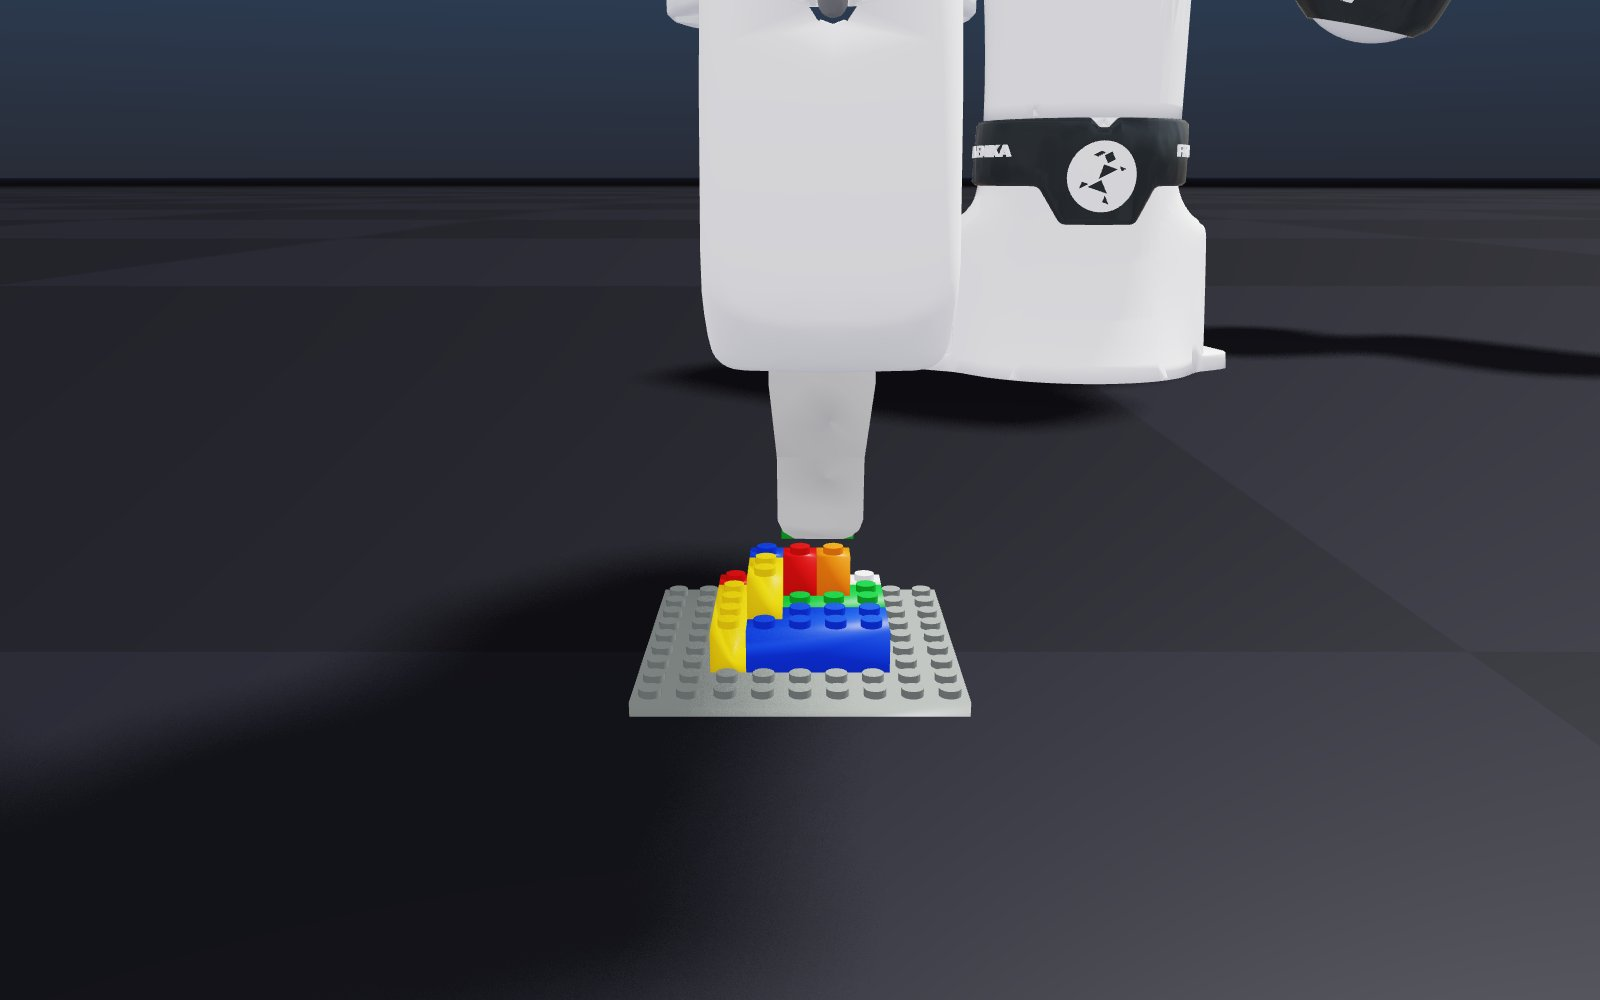
\includegraphics[width=\linewidth]{sim_p_drop9.jpg}\caption{Lowering the boxed-in 2$\times$2.}\end{subfigure}\hfill
\begin{subfigure}{.32\linewidth}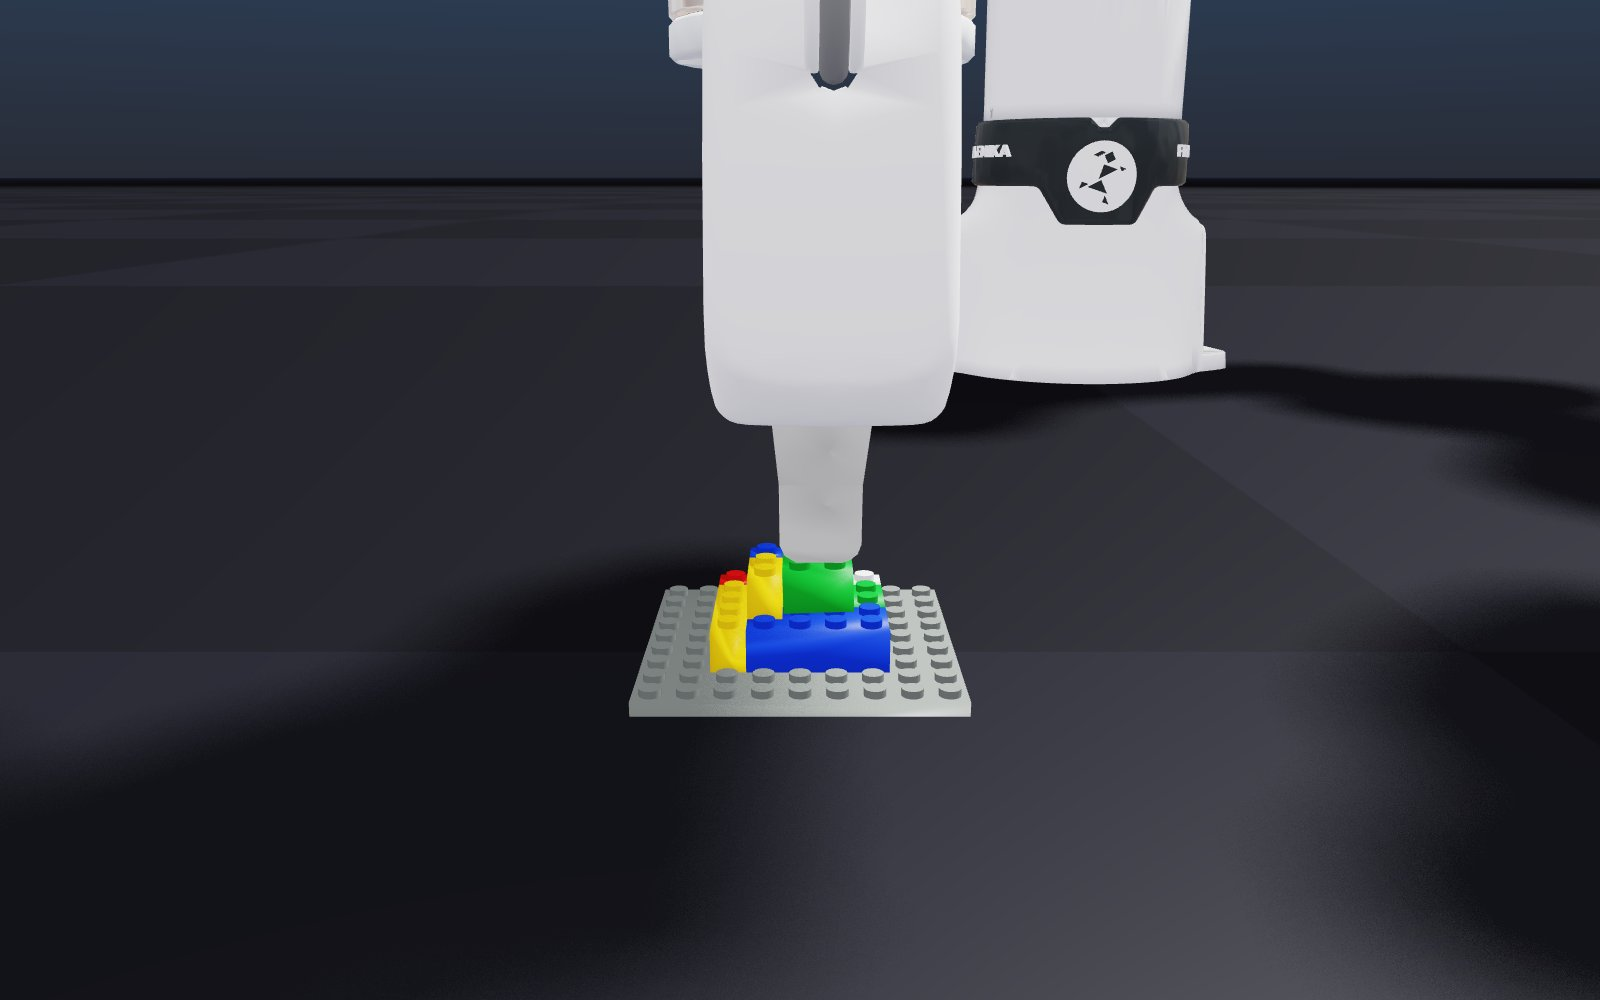
\includegraphics[width=\linewidth]{sim_p_press9.jpg}\caption{Pressing with closed fingertips.}\end{subfigure}\hfill
\begin{subfigure}{.32\linewidth}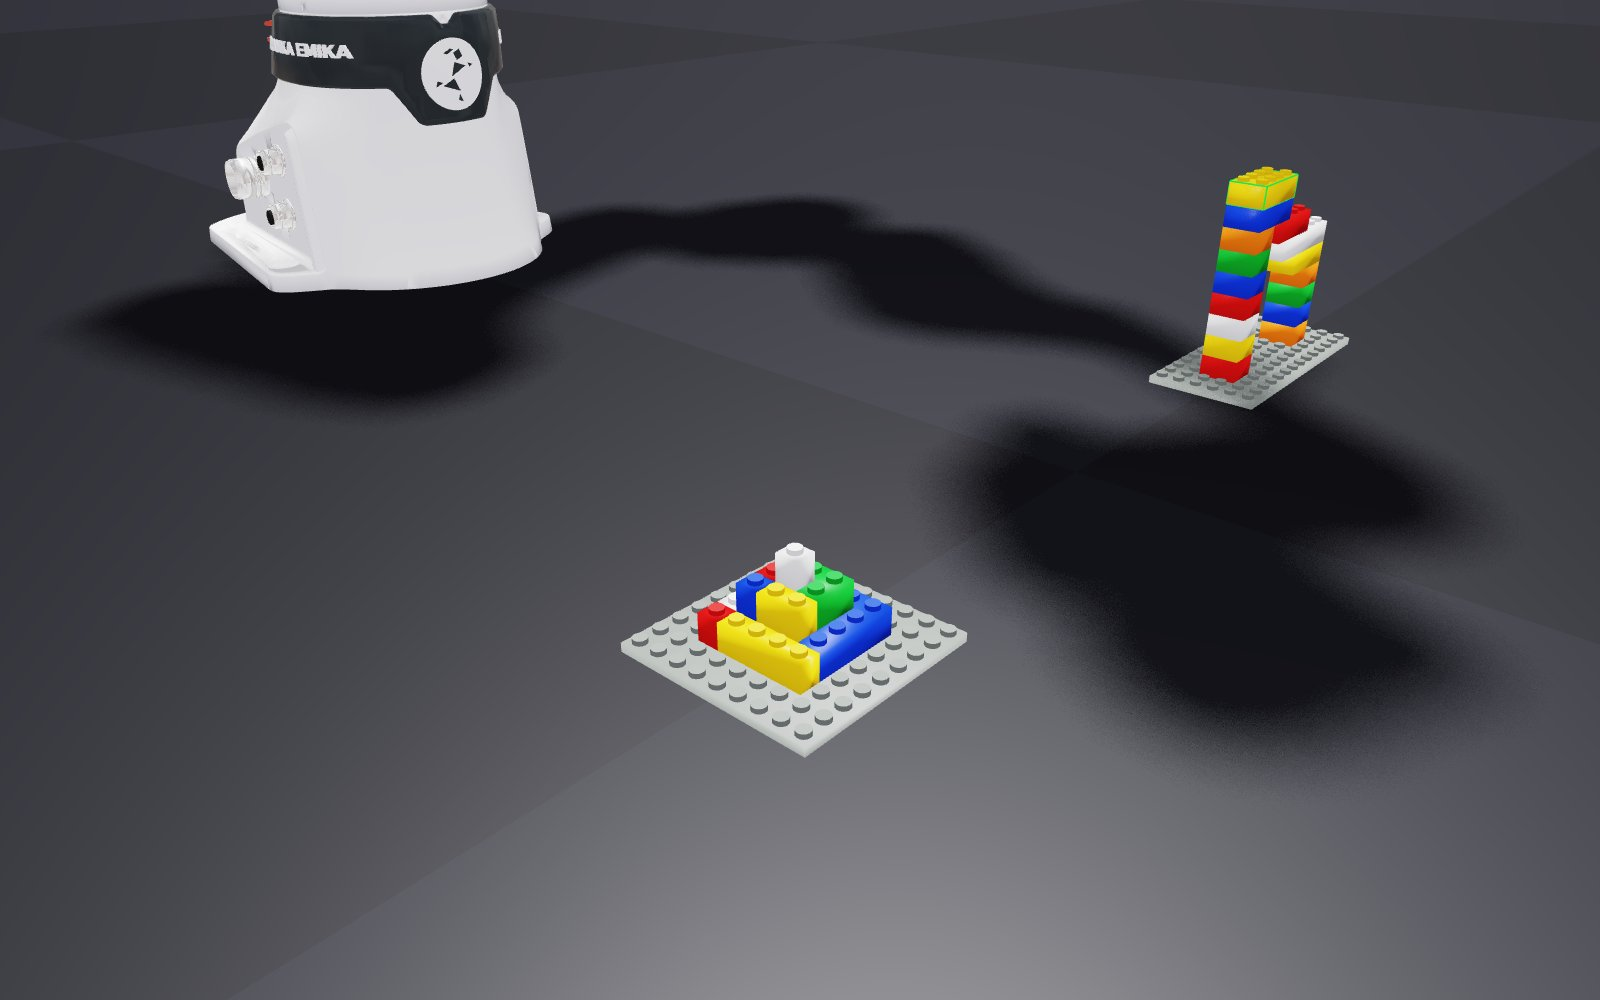
\includegraphics[width=\linewidth]{sim_p_fin.jpg}\caption{Finished pyramid.}\end{subfigure}
\caption{Drop-and-press on the user's pyramid (step 9).}
\end{figure}

\subsection{Tight slots: scripted wriggle}
The arch crown drops into a slot between two placed bricks with about 0.1\,mm
of play per side. Straight insertion tends to jam on one side. Such steps
replay a scripted search taken from the team's tight-fit study: small lateral
motions (0.1\,mm) and rocking (0.1$^\circ$) while descending, then a longer
final press. A learned (reinforcement learning) wriggle was trained in the
team's MuJoCo study but did not beat the scripted one, so the scripted version
is used.

\begin{figure}[H]
\centering
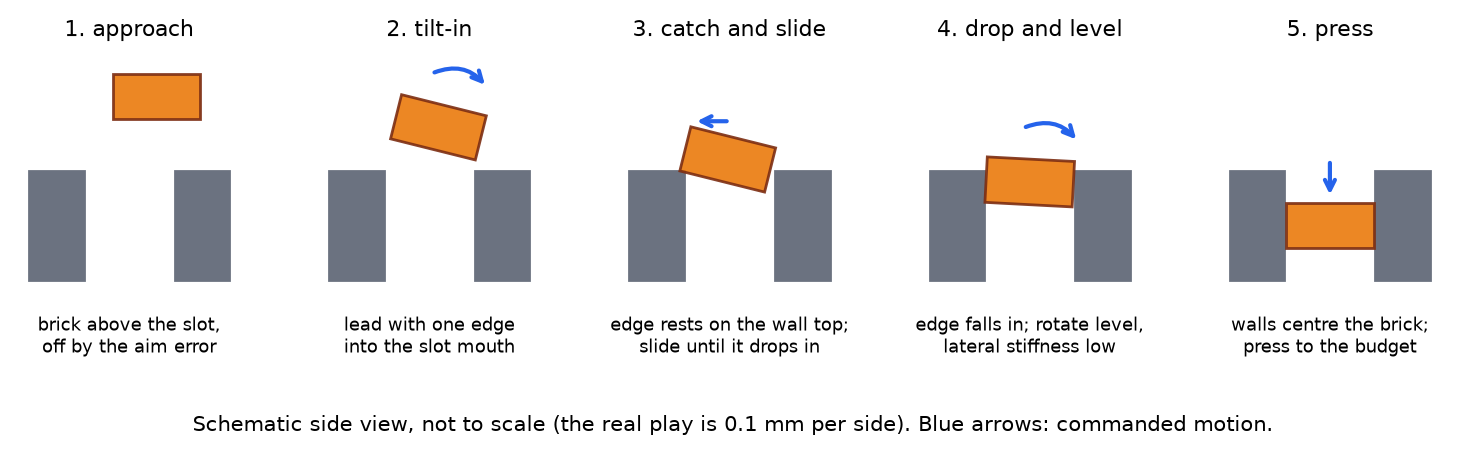
\includegraphics[width=.92\linewidth]{wriggle_primitive.png}
\caption{The wriggle idea (schematic, from the tight-fit study): tilt in, catch an
edge, slide, level, press.}
\end{figure}

\subsection{The supporting grasp}
When a step needs support, the helper arm:
\begin{enumerate}[nosep]
\item searches up to 8 support configurations generated by the support planner
      (planned pose, other lean angles, other heights and columns), accepting
      only ones whose predicted support is \emph{no worse} than the plan's;
\item for each, checks its own approach and finger-closing sweep, \emph{and} the
      builder's whole path including the carried brick's insertion corridor,
      against its measured joints, with fingers open and closed;
\item approaches the last 10\,mm slowly (5\,mm/s) with open fingers, closes, and
      confirms that \emph{both} fingers measure contact force;
\item holds its measured joints until the builder has inserted, released and moved away.
\end{enumerate}
In the validated run a candidate pose was rejected 6 times for a real reason
(for example ``closed finger 0.90\,mm from brick A\_b\_000'' or ``helper obstructs
the carried brick's insertion corridor by 0.74\,mm'') and an alternative was
accepted each time. Measured grip force was 13.0--14.0\,N per finger against
the 14.3\,N the plan assumed.

\subsection{Recovering from a failed support attempt}\label{sec:recovery}
The checks above all happen \emph{before} the helper closes its fingers. The
harder stud-fit runs (\S\ref{sec:studfit}) showed four ways an attempt can still
go wrong after that point. Each one used to end the build or push the
structure out of place. The support search now treats each as a bad candidate
and moves on:
\begin{itemize}[nosep]
\item \textbf{The closed hand blocks the builder.} After closing, the measured hold
      can sit deeper than the open-hand check predicted. The builder's approach is
      re-checked against the \emph{closed} helper before the builder may move; if it
      is blocked, the helper opens, retreats and tries the next pose.
\item \textbf{One finger misses.} A grip is only ``held'' when both fingers feel
      force; in stud-fit mode every brick the plan meant to grip must also be in
      contact. Otherwise the helper retreats and tries the next pose.
\item \textbf{The guarded approach stops on contact (guard stop).} The helper no
      longer closes into the scrape. It pulls back 2.5$\times$ further than usual,
      without first opening its fingers there, and tries a column at least 12\,mm
      away before nearby ones.
\item \textbf{A pose that failed is not retried}, including its 180$^\circ$ wrist twin,
      which grips the same brick face.
\end{itemize}

\begin{figure}[H]
\centering
\begin{subfigure}{.32\linewidth}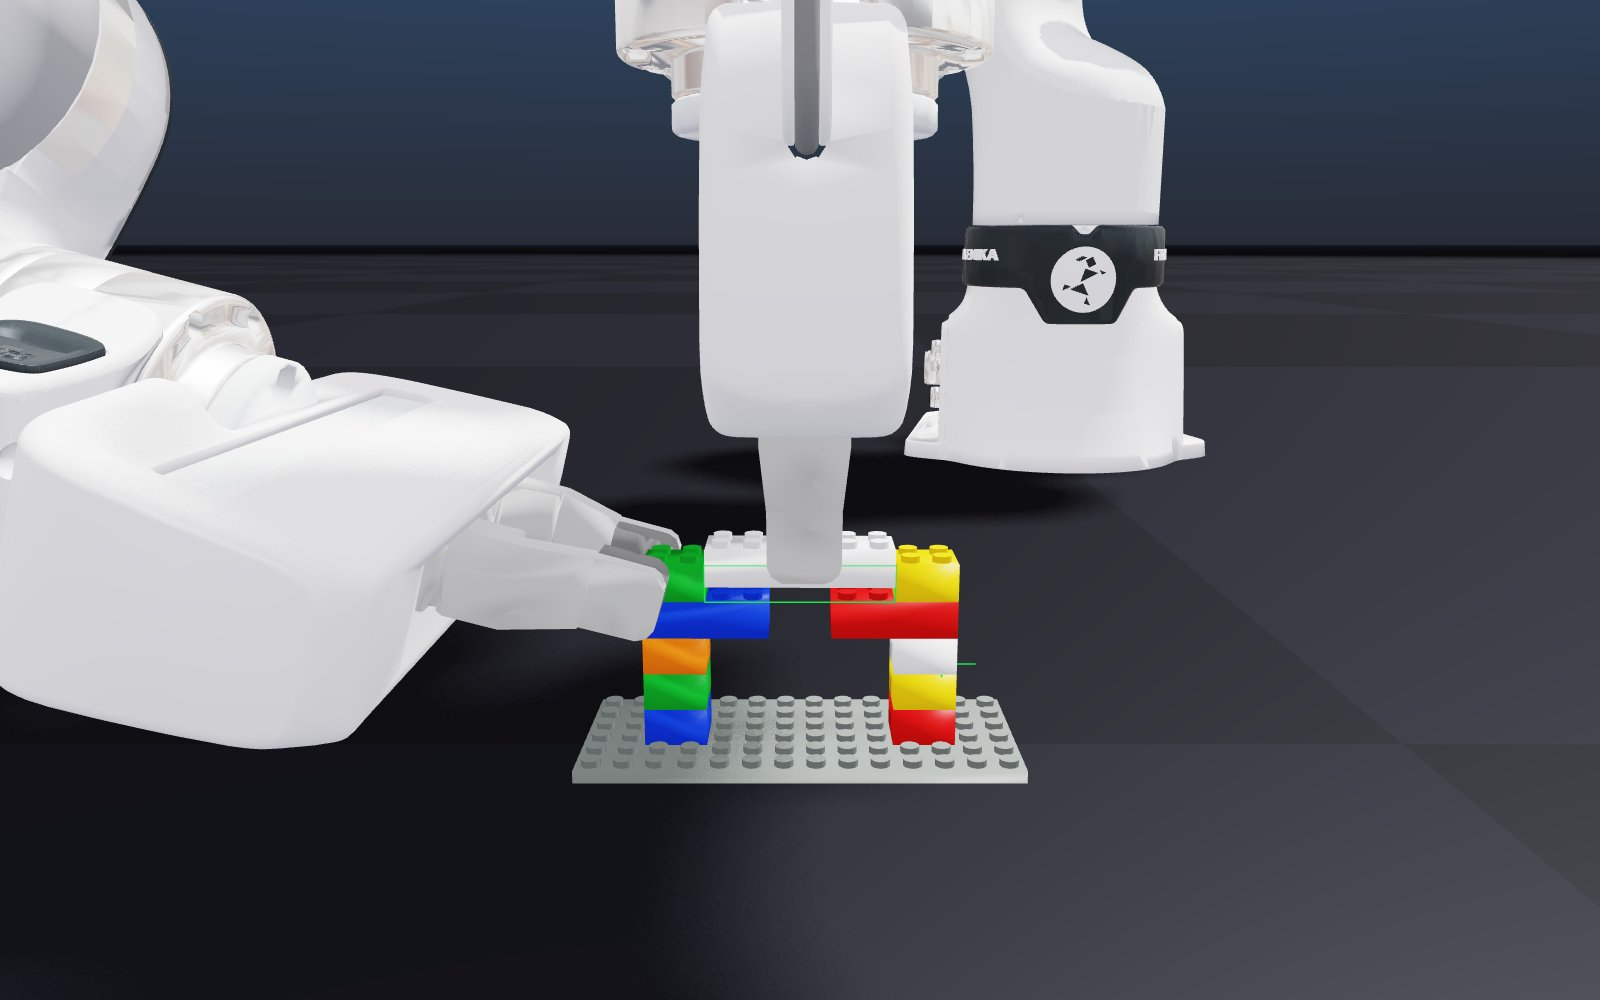
\includegraphics[width=\linewidth]{sim_a_sup10_side.jpg}\caption{Arch step 10: B holds, A presses the crown.}\end{subfigure}\hfill
\begin{subfigure}{.32\linewidth}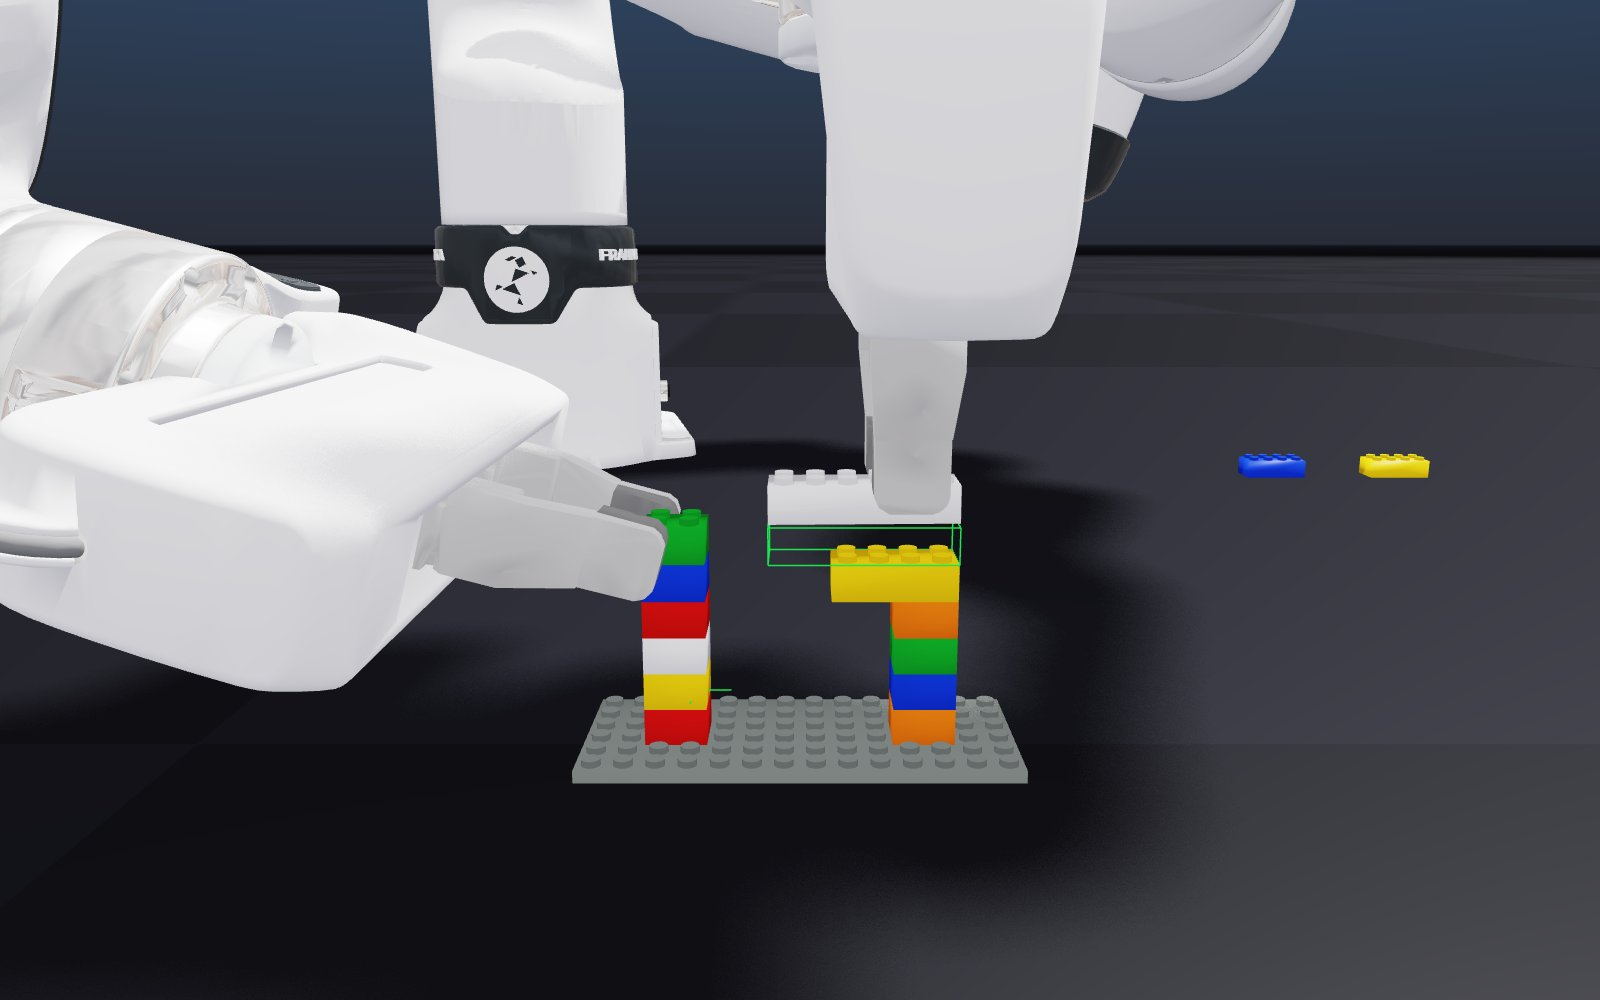
\includegraphics[width=\linewidth]{sim_a_sup11_side.jpg}\caption{S3 step 11: A holds, B places the corbel.}\end{subfigure}\hfill
\begin{subfigure}{.32\linewidth}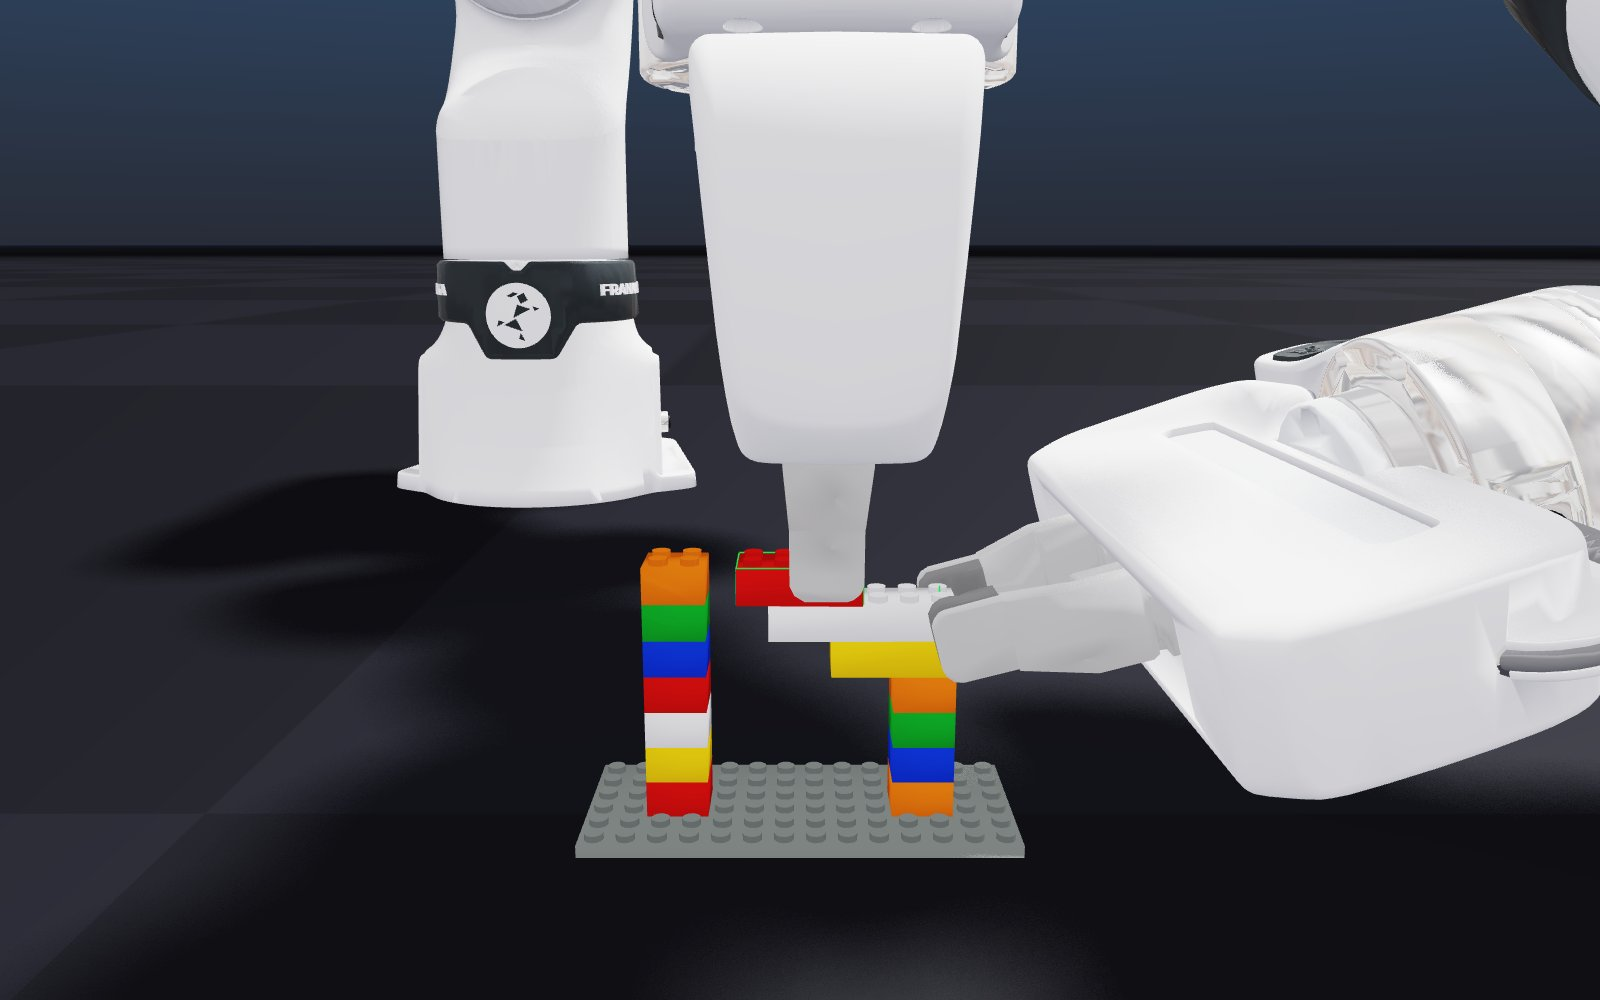
\includegraphics[width=\linewidth]{sim_a_sup13_side.jpg}\caption{S3 step 13: A grips the left pier top.}\end{subfigure}
\caption{Reciprocal support in the validated run. The helper's hand comes in from the side, leaning away from the builder's hand.}
\end{figure}

\why{Each manipulation behaviour is a small script with a measurable check,
rather than a learned policy, because the checks (finger clearance, contact force,
snap error) make failures visible and fixable. The fallback order goes from the
grip the planner preferred to the least preferred, so the plan's intent is kept
whenever it is physically possible. Learning was tried for insertion and lost
to the scripted wriggle, and the supervisor's scope did not require it.}

% =====================================================================
\section{Collision avoidance}\label{sec:collision}

\keyidea{Every arm is a chain of spheres, every obstacle is a box; nothing may come
within 1\,mm unless the contact is intended, and two arms move together only
when the space each will sweep has been reserved and does not overlap.}

Safety is layered: a problem missed by one layer is caught by the next.

\begin{figure}[H]
\centering
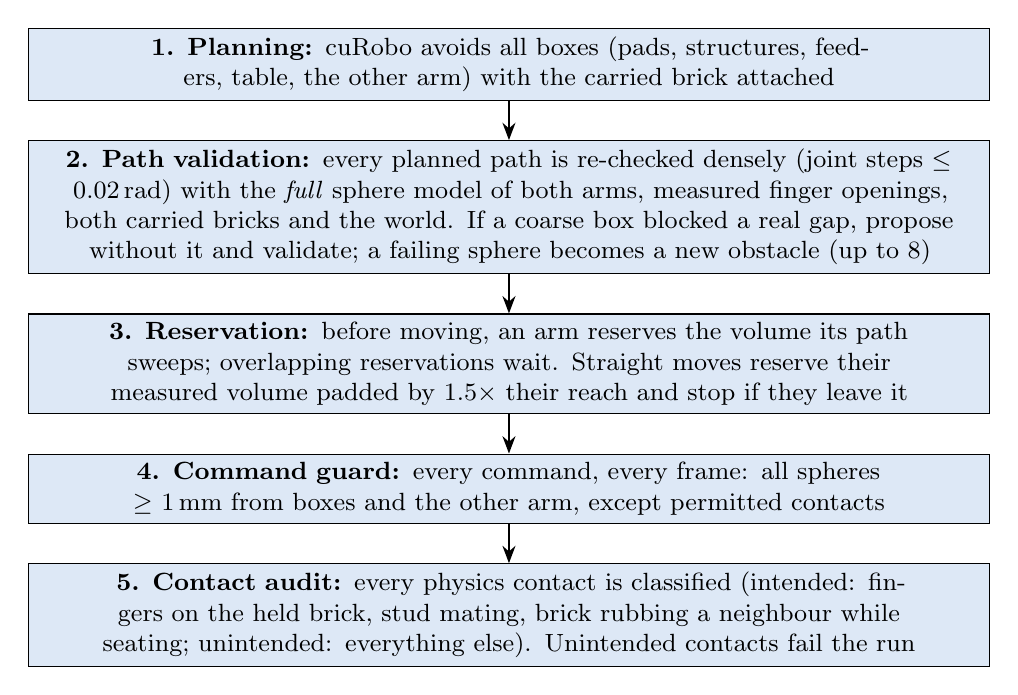
\begin{tikzpicture}[flow]
\node[step=120mm] (l1) {\textbf{1. Planning:} cuRobo avoids all boxes (pads, structures, feeders, table, the other arm) with the carried brick attached};
\node[step=120mm, below=of l1] (l2) {\textbf{2. Path validation:} every planned path is re-checked densely (joint steps $\le$ 0.02\,rad) with the \emph{full} sphere model of both arms, measured finger openings, both carried bricks and the world. If a coarse box blocked a real gap, propose without it and validate; a failing sphere becomes a new obstacle (up to 8)};
\node[step=120mm, below=of l2] (l3) {\textbf{3. Reservation:} before moving, an arm reserves the volume its path sweeps; overlapping reservations wait. Straight moves reserve their measured volume padded by 1.5$\times$ their reach and stop if they leave it};
\node[step=120mm, below=of l3] (l4) {\textbf{4. Command guard:} every command, every frame: all spheres $\ge$ 1\,mm from boxes and the other arm, except permitted contacts};
\node[step=120mm, below=of l4] (l5) {\textbf{5. Contact audit:} every physics contact is classified (intended: fingers on the held brick, stud mating, brick rubbing a neighbour while seating; unintended: everything else). Unintended contacts fail the run};
\foreach \u/\v in {l1/l2,l2/l3,l3/l4,l4/l5} \draw[arr] (\u) -- (\v);
\end{tikzpicture}
\caption{The five layers of collision protection.}
\end{figure}

\subsection{The sphere model}
The robot model used by cuRobo describes each link with a set of spheres. The
clearance checker uses the same \emph{full} set, moves the finger spheres to the
measured finger opening, and adds the carried brick as spheres inscribed in its
box (so the check never overestimates the gap). Distances between two arms are
computed sphere-to-sphere, with a bounding-box pre-test per link pair to skip
far-apart links; distances to the world use oriented boxes.

\subsection{Sharing the space: reservations}
Two arms planned separately can each be safe against where the \emph{other}
arm is now, yet collide when both move. Instead of a joint 14-joint planner, the
project uses conservative \textbf{space reservations}:
\begin{itemize}
\item A planned path reserves the axis-aligned boxes swept by each link's spheres
      along the whole path.
\item A Cartesian move reserves the arm's measured volume padded by 1.5$\times$ its
      hand travel plus allowances for wrist turn and 10\,mm; if the arm ever
      leaves it while the other arm moves, it stops.
\item A new reservation is admitted only if it is at least 25\,mm away from the
      other arm's active one; otherwise the arm waits at a checked pose.
\end{itemize}
With this, both builders moved simultaneously for 1{,}643 frames in the
validated run (compared with 260 frames when every contact move took a global
lock), with a minimum measured clearance of 1.21\,mm.

\why{Spheres make distance checks fast and conservative, and the same model is
used by the planner and the checker, so they cannot disagree about geometry.
Reservations keep each arm's own proven planner and add coordination on top, a
much smaller and more testable change than planning both arms jointly. The
1\,mm floor is never relaxed; fallbacks only change how a path is
\emph{proposed}, never how it is \emph{accepted}. Sampled checks are not a
continuous-collision proof, which is why the physics contact audit exists as
the final layer.}

% =====================================================================
\section{Task execution and completion}\label{sec:execution}

\keyidea{A small deterministic coordinator lets each arm work through its own plan,
pauses one to help the other when a step needs support (arm A first on a tie),
and a strict snap check decides when each brick, and the whole task, is done.}

\subsection{The coordinator}\label{sec:coord}
The coordinator (\texttt{dual\_coordinator.py}) acts only at step boundaries. Each
arm has its own plan, step counter and status. Every frame it is asked who may
start what:
\begin{itemize}
\item \textbf{No support needed:} each idle arm starts its next step; both may build at once.
\item \textbf{A support request} is recorded \emph{before} the builder picks up its
      brick. The coordinator waits until \emph{both} arms are idle (the helper
      finishes its current placement and retracts; nothing in flight is interrupted).
\item \textbf{Tie:} if both arms have pending requests, A is served first and B's
      request is kept and served next, so it cannot starve.
\item \textbf{Completed builder:} an arm that has finished its own structure stays
      available as a helper.
\item \textbf{Don't run ahead (added after the validated runs):} an arm that is
      already ahead of the other in step count does not start a new step of its own
      while the other arm's \emph{next} step needs support. Without this rule, the
      pyramid arm, already ahead, started a slow drop-and-press just as S3's
      next step needed a helper, and that S3 brick later missed its snap check.
\end{itemize}
Because requests are collected before pickup and only granted when both arms are
idle, the state ``both arms hold a brick and each waits for the other to help''
cannot occur.

\begin{figure}[H]
\centering
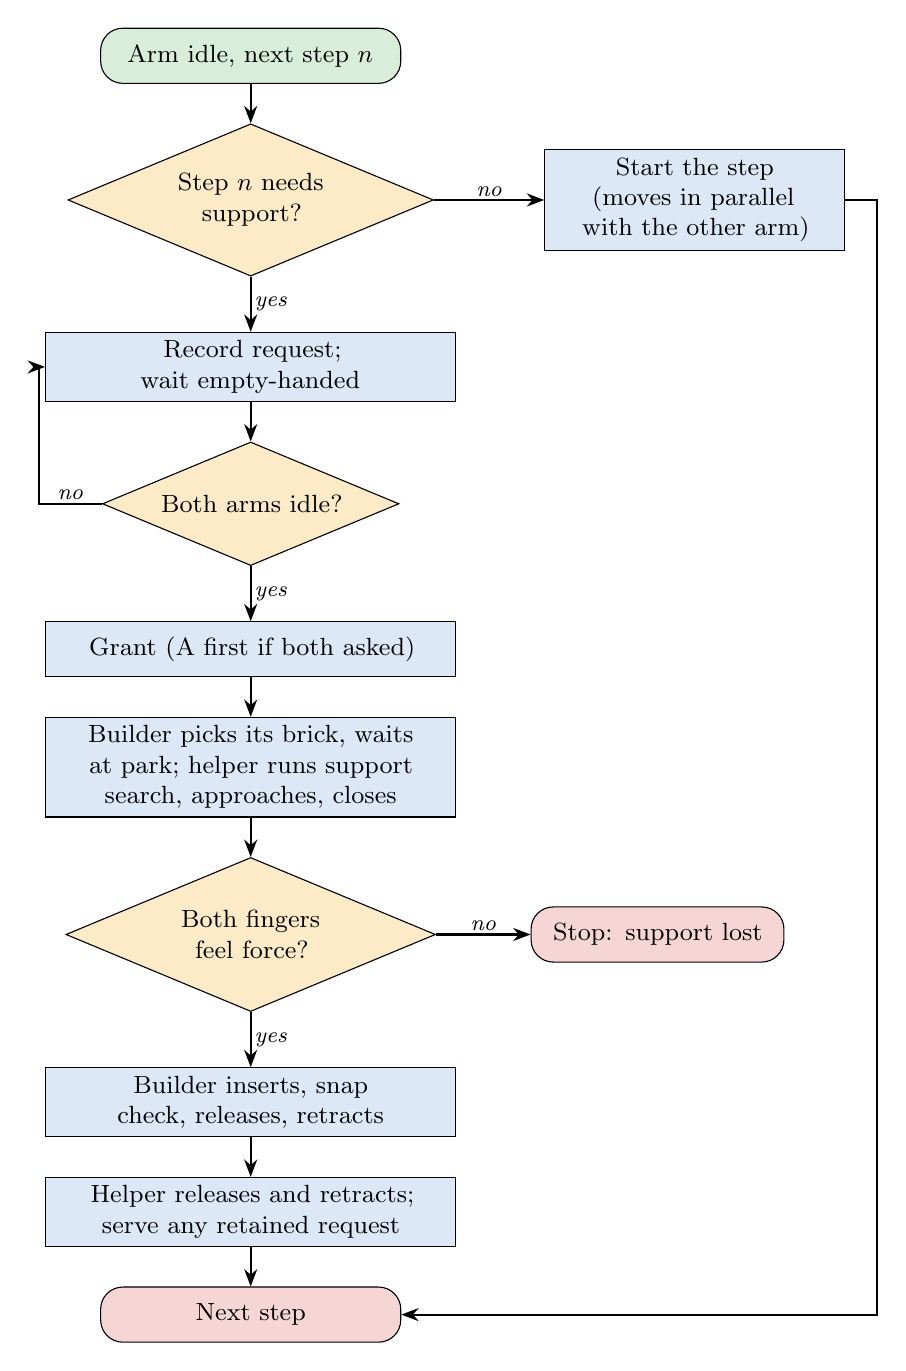
\begin{tikzpicture}[flow]
\node[start=36mm] (s) {Arm idle, next step $n$};
\node[ask=28mm, below=of s] (q1) {Step $n$ needs support?};
\node[step=36mm, right=14mm of q1] (go) {Start the step (moves in parallel with the other arm)};
\node[step=50mm, below=of q1, yshift=-2mm] (req) {Record request; wait empty-handed};
\node[ask=30mm, below=of req] (q2) {Both arms idle?};
\node[step=50mm, below=of q2, yshift=-2mm] (grant) {Grant (A first if both asked)};
\node[step=50mm, below=of grant] (b1) {Builder picks its brick, waits at park; helper runs support search, approaches, closes};
\node[ask=30mm, below=of b1] (q3) {Both fingers feel force?};
\node[stop=30mm, right=12mm of q3] (f) {Stop: support lost};
\node[step=50mm, below=of q3, yshift=-2mm] (b2) {Builder inserts, snap check, releases, retracts};
\node[step=50mm, below=of b2] (b3) {Helper releases and retracts; serve any retained request};
\node[stop=36mm, below=of b3] (e) {Next step};
\draw[arr] (s)--(q1);
\draw[arr] (q1)-- node[lab,above]{no} (go);
\draw[arr] (q1)-- node[lab,right]{yes} (req);
\draw[arr] (req)--(q2);
\draw[arr] (q2.west) -- node[lab,above]{no} ++(-8mm,0) |- (req.west);
\draw[arr] (q2)-- node[lab,right]{yes} (grant);
\draw[arr] (grant)--(b1); \draw[arr] (b1)--(q3);
\draw[arr] (q3)-- node[lab,above]{no} (f);
\draw[arr] (q3)-- node[lab,right]{yes} (b2);
\draw[arr] (b2)--(b3); \draw[arr] (b3)--(e);
\draw[arr] (go.east) -- ++(4mm,0) |- (e.east);
\end{tikzpicture}
\caption{The support handshake.}
\end{figure}

\begin{figure}[H]
\centering
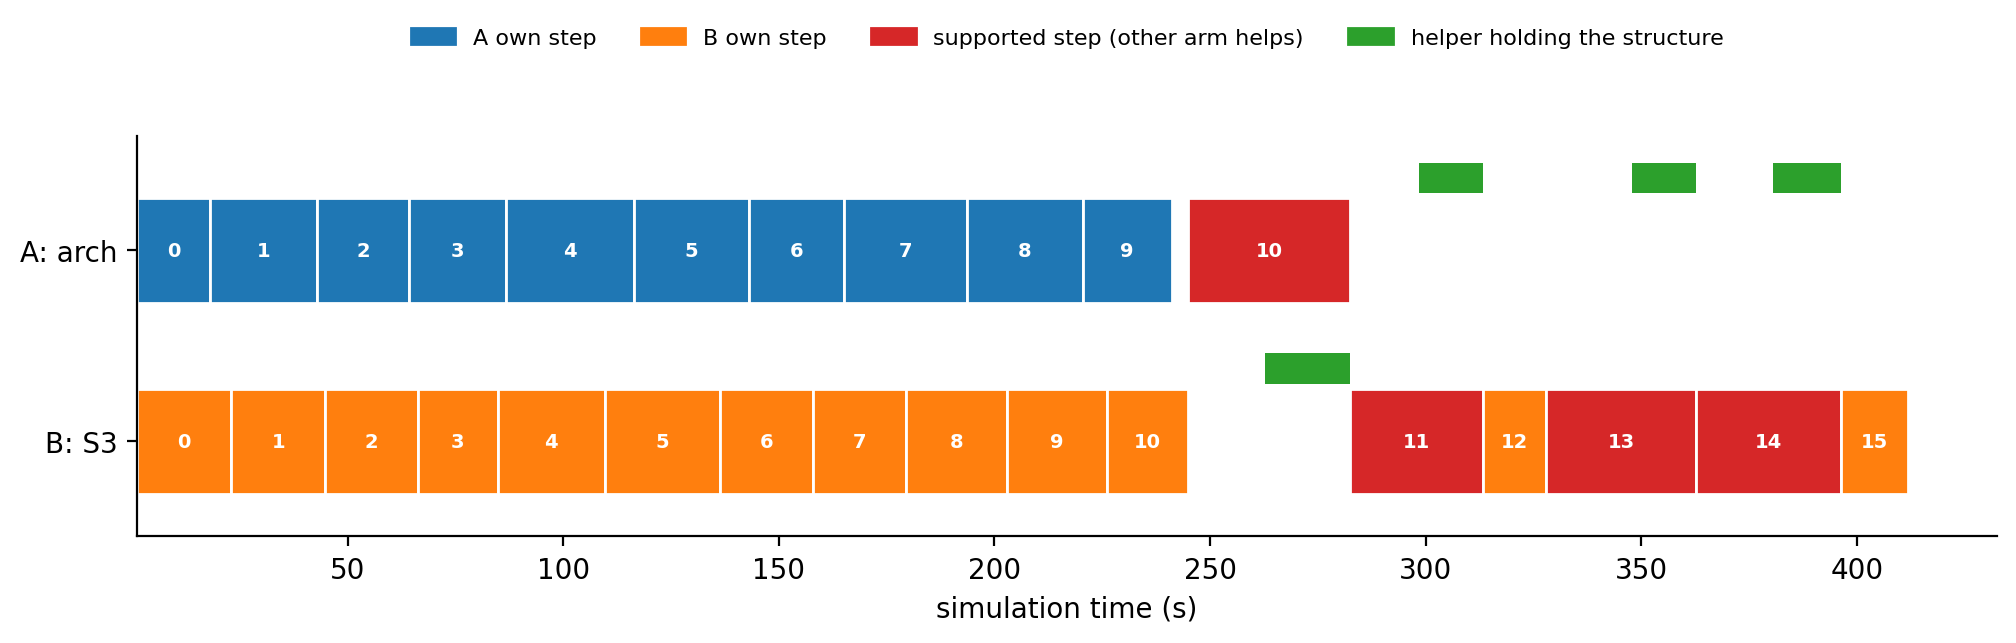
\includegraphics[width=\linewidth]{timeline_arch_s3.png}
\caption{Timeline of the validated run, from the saved scheduler events. Steps
0--9 of both structures overlap in time. At 241\,s A asks for help (step 10);
at 245\,s B asks too (step 11). A is served first; B's request is served next,
then B's steps 13 and 14 with A, which has already finished the arch, helping.}
\label{fig:timeline}
\end{figure}

\subsection{When is a brick placed? The snap check}\label{sec:done}
At the end of each press the brick's real pose is compared with its target:

\begin{center}
\small
\begin{tabular}{@{}lc@{}}
\toprule
Quantity & Must be below \\
\midrule
sideways distance & 2\,mm \\
height difference & 1.5\,mm \\
wrong rotation (yaw) & 5$^\circ$ \\
tilt & 5$^\circ$ \\
\bottomrule
\end{tabular}
\end{center}
If all four pass, the clutch welds switch on and the step is complete. If any
fails, the run stops with \texttt{gate\_miss}; a mistake is never hidden by
continuing.

\begin{figure}[H]
\centering
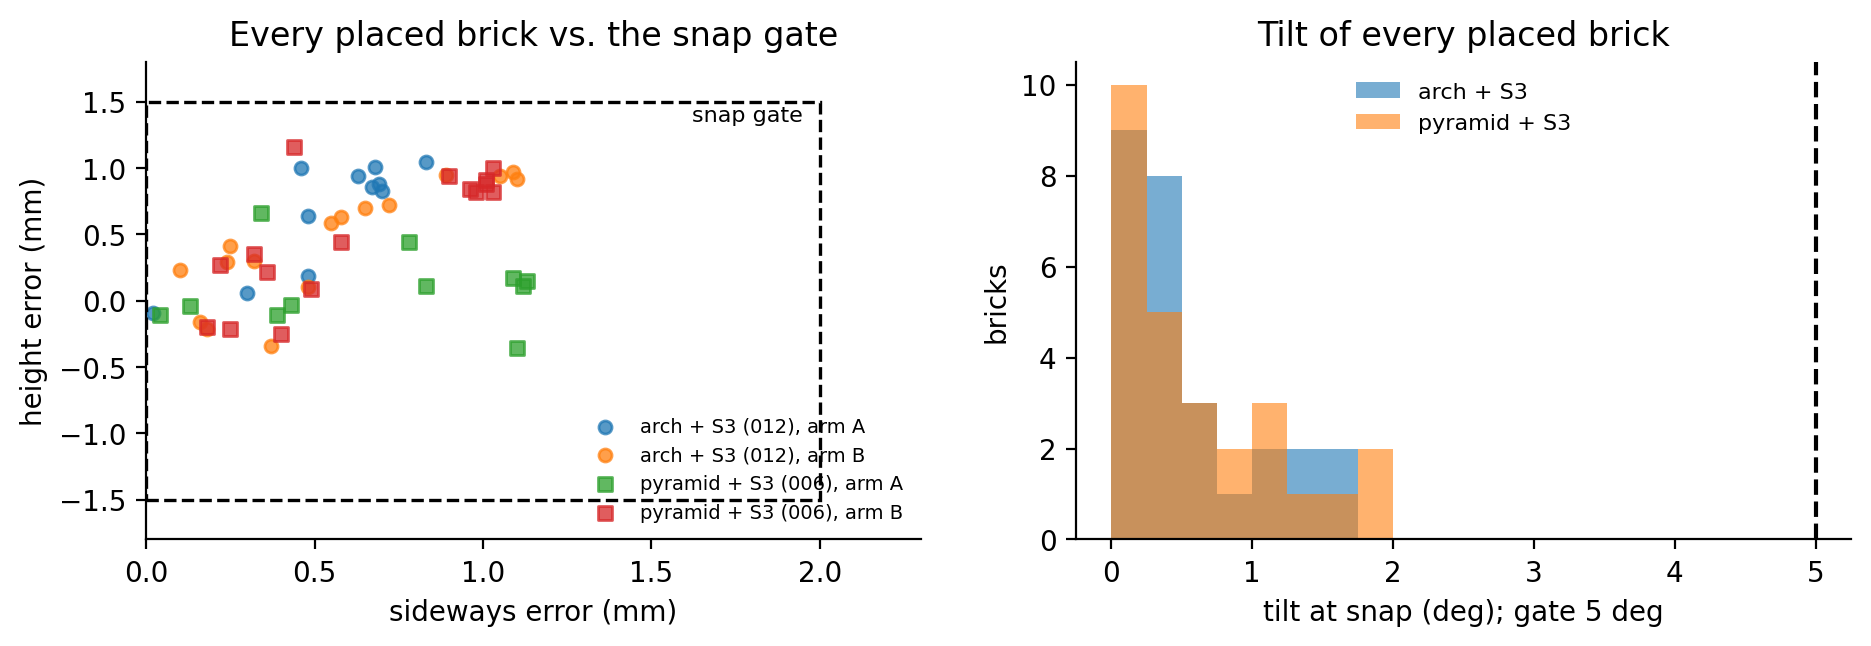
\includegraphics[width=\linewidth]{snap_accuracy.png}
\caption{Every one of the 54 bricks in both full runs, against the snap check.
All lie well inside: at most 1.13\,mm sideways, 1.16\,mm in height and
1.92$^\circ$ of tilt.}
\end{figure}

\subsection{When is the task complete? Independent verification}
A run is complete when both coordinator builds have finished every step. The
claim is then checked by a separate program, \texttt{Kean/verify\_dual.py}, which
reads only the saved files (plans, events, contacts, recording, provenance) and
checks that:
\begin{itemize}[nosep]
\item each arm completed every step of its own plan, in order, and every step has recorded insertion and stud-mating evidence;
\item every generated support was requested before pickup, granted in A-first order with the losing request served next, held without the helper moving, with measured force on both fingers, and released in order; no request was left unserved;
\item both arms actually moved as builders at the same time (parallel frames recorded);
\item there were no arm--arm contacts, unintended contacts, invalid stud contacts, broken joints or execution failures;
\item the run is not a diagnostic shortcut (no pre-placed bricks).
\end{itemize}
Each run also saves its provenance (code revision, file hashes, configuration)
next to the results.
Both final runs pass (exit code 0).

\begin{figure}[H]
\centering
\begin{subfigure}{.32\linewidth}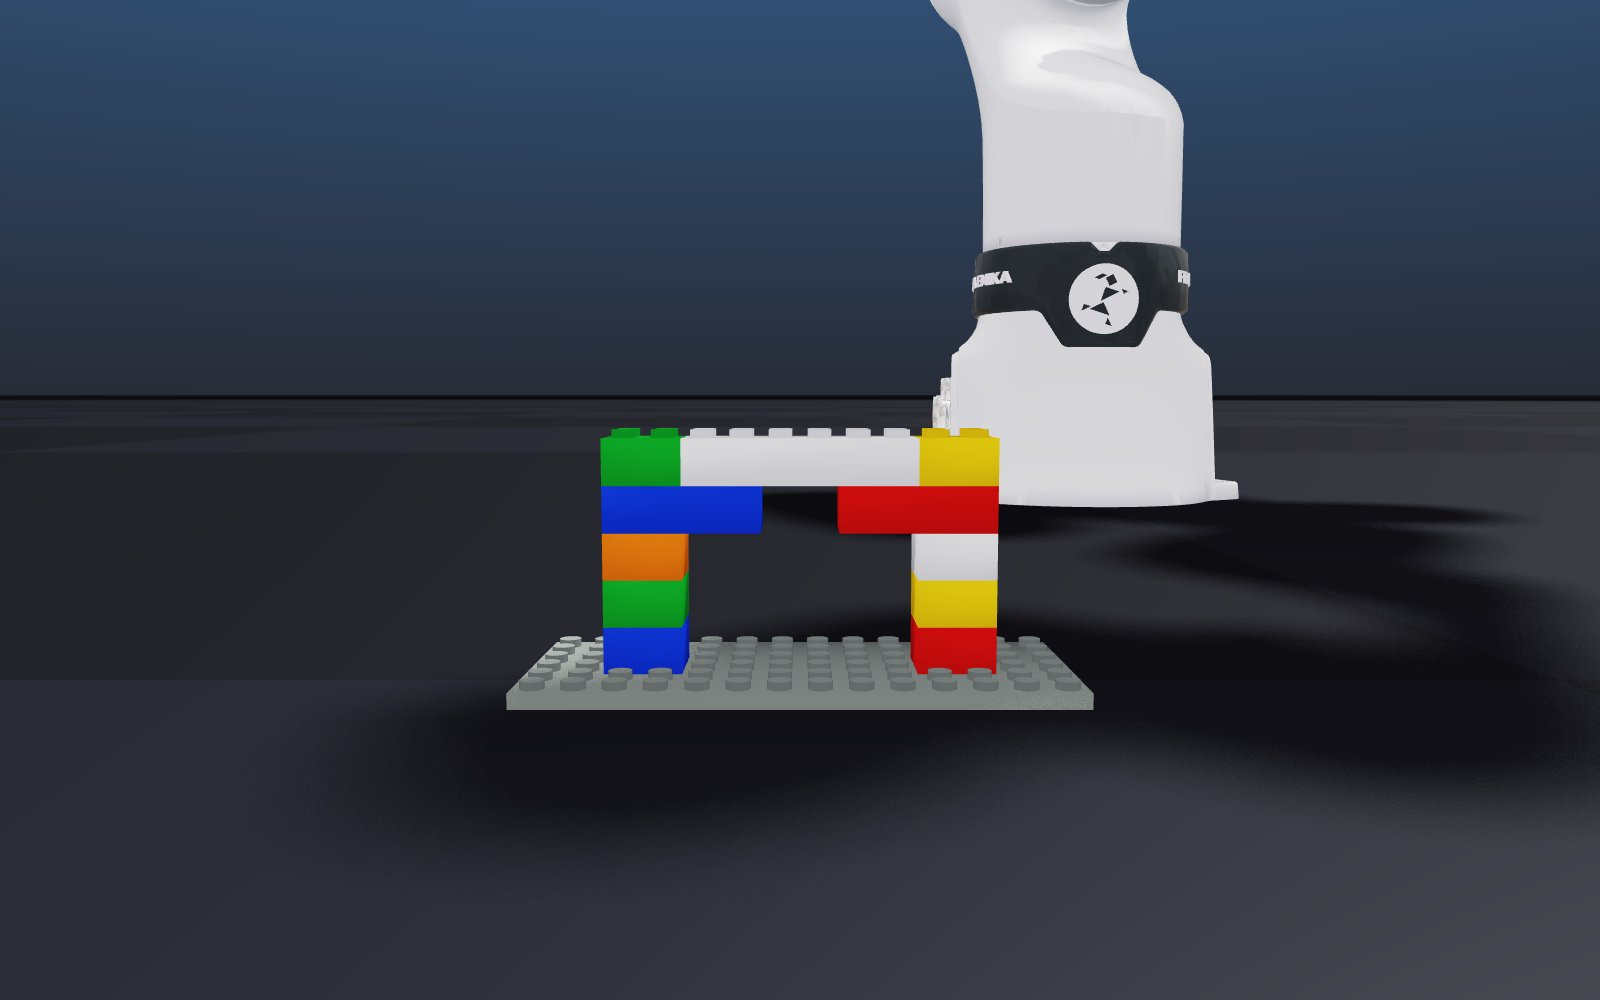
\includegraphics[width=\linewidth]{sim_a_fin_arch_side.jpg}\caption{Arch.}\end{subfigure}\hfill
\begin{subfigure}{.32\linewidth}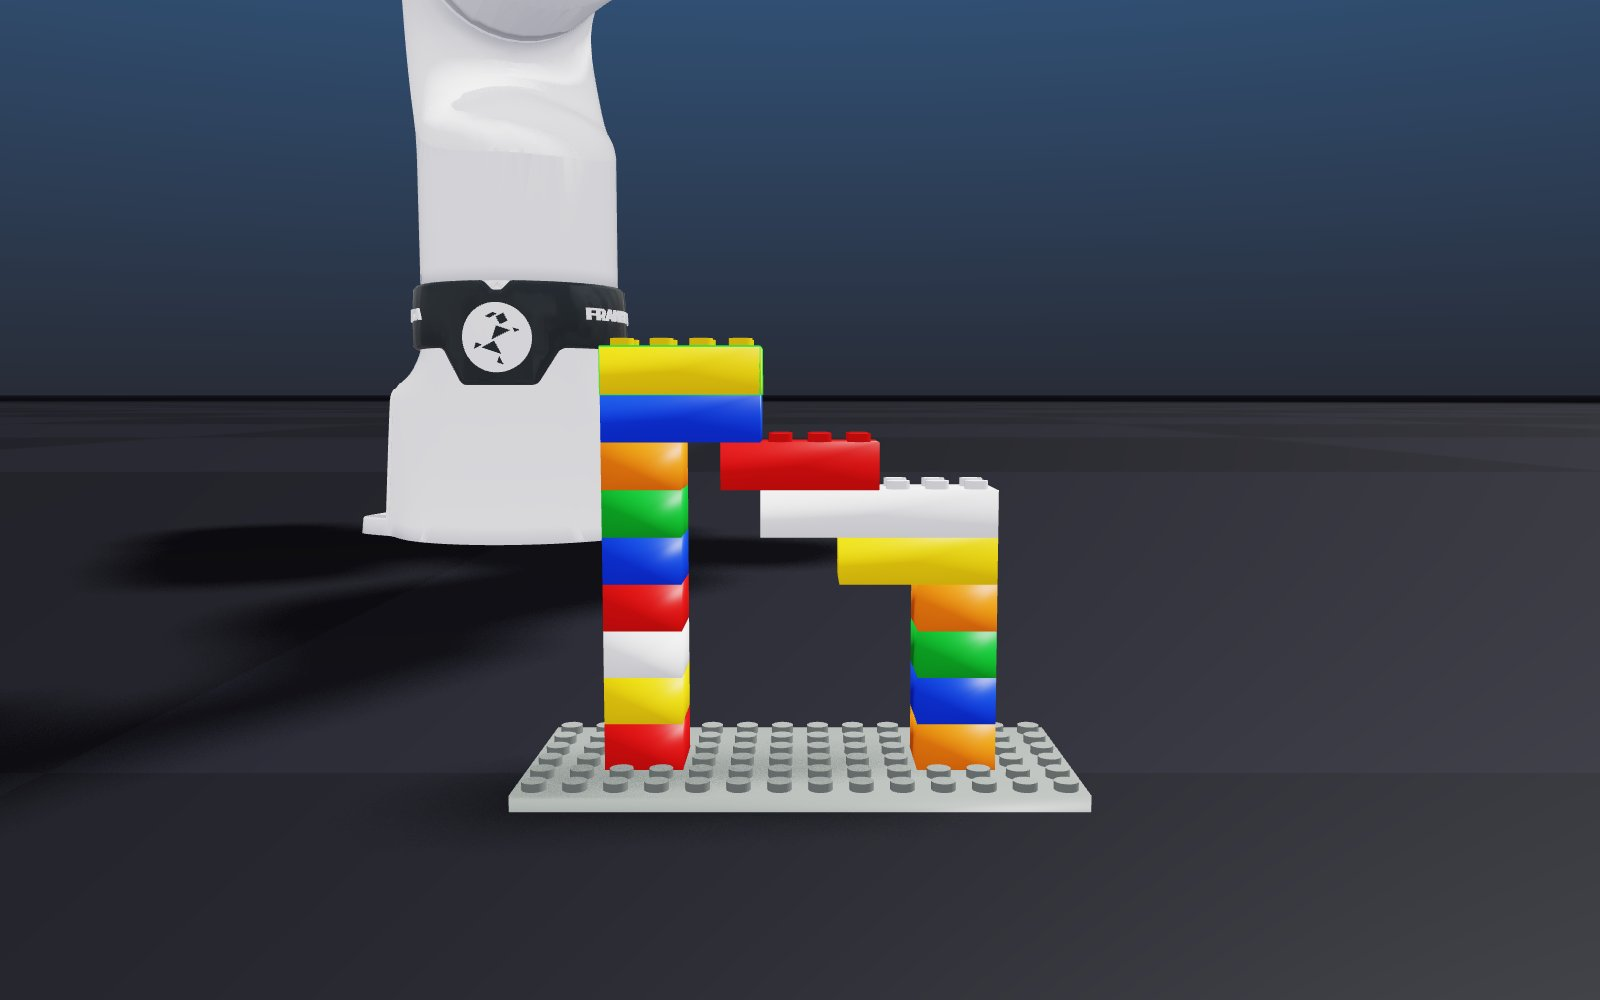
\includegraphics[width=\linewidth]{sim_a_fin_s3_side.jpg}\caption{S3 corbelled bridge.}\end{subfigure}\hfill
\begin{subfigure}{.32\linewidth}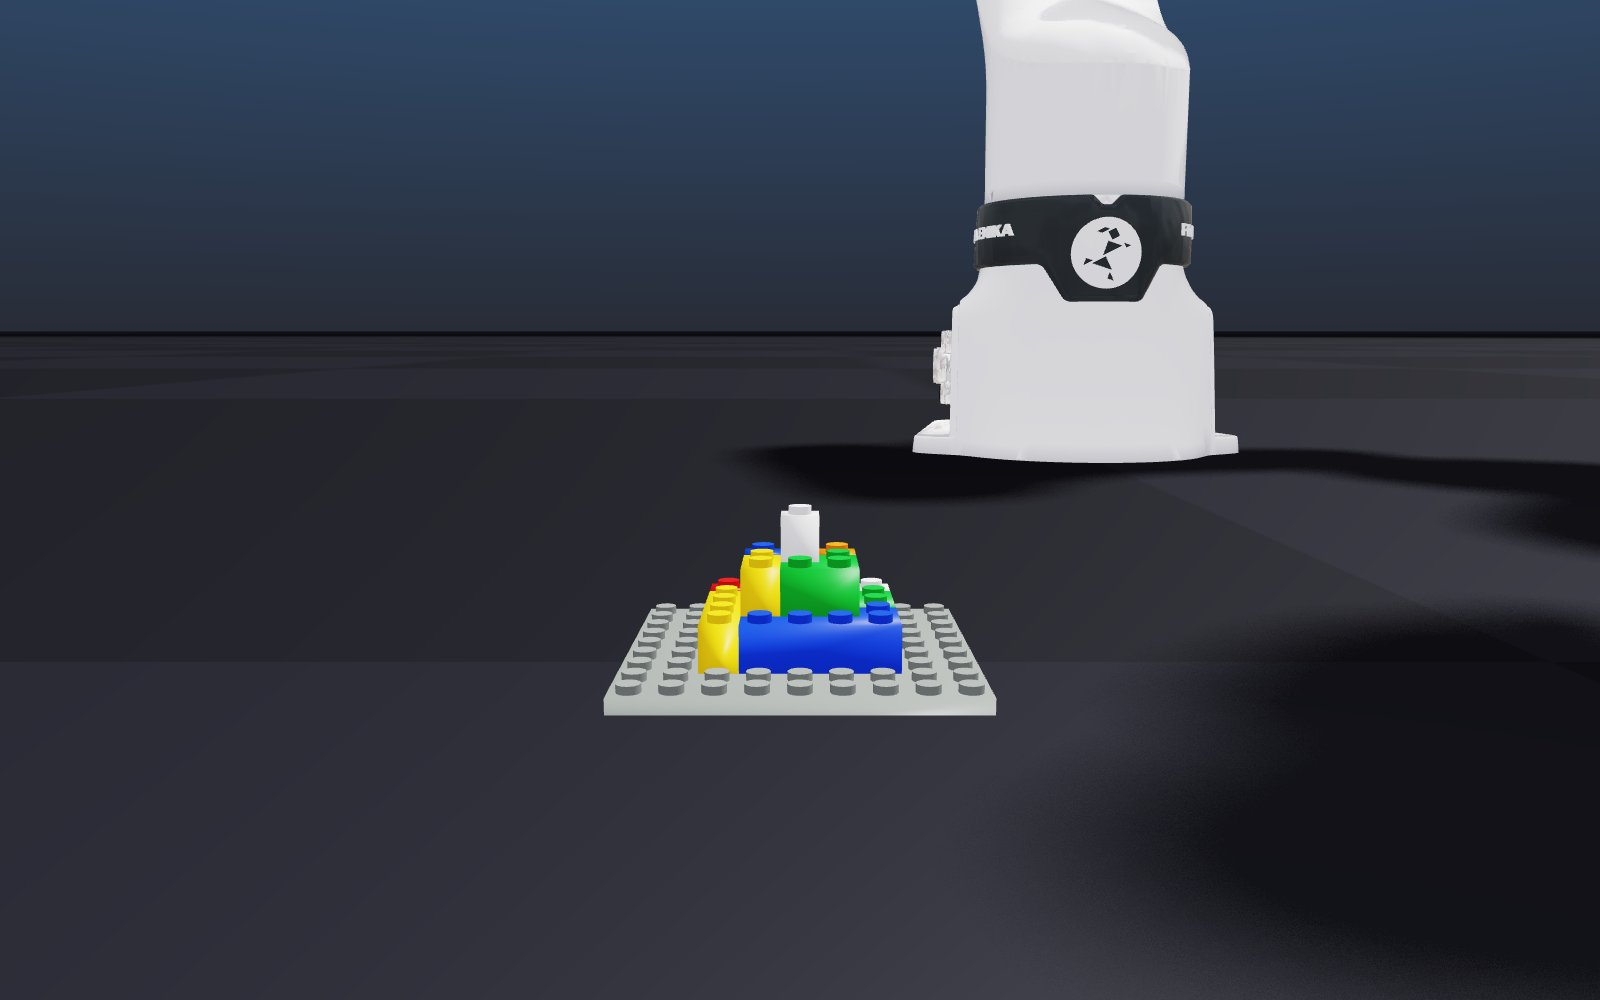
\includegraphics[width=\linewidth]{sim_p_fin_side.jpg}\caption{Pyramid (user drawing).}\end{subfigure}
\caption{The three structures built from their inputs (Figure~\ref{fig:inputs}).}
\end{figure}

\why{A deterministic, step-boundary coordinator is small (about 70 lines), easy to
unit-test for every case (single request, tie, retained request, role reversal,
finished builder), and cannot deadlock by construction. The snap check makes
``placed'' a measurable fact. The separate verifier means a run is judged from
evidence, not from the program's own opinion of itself.}

\begin{figure}[H]
\centering
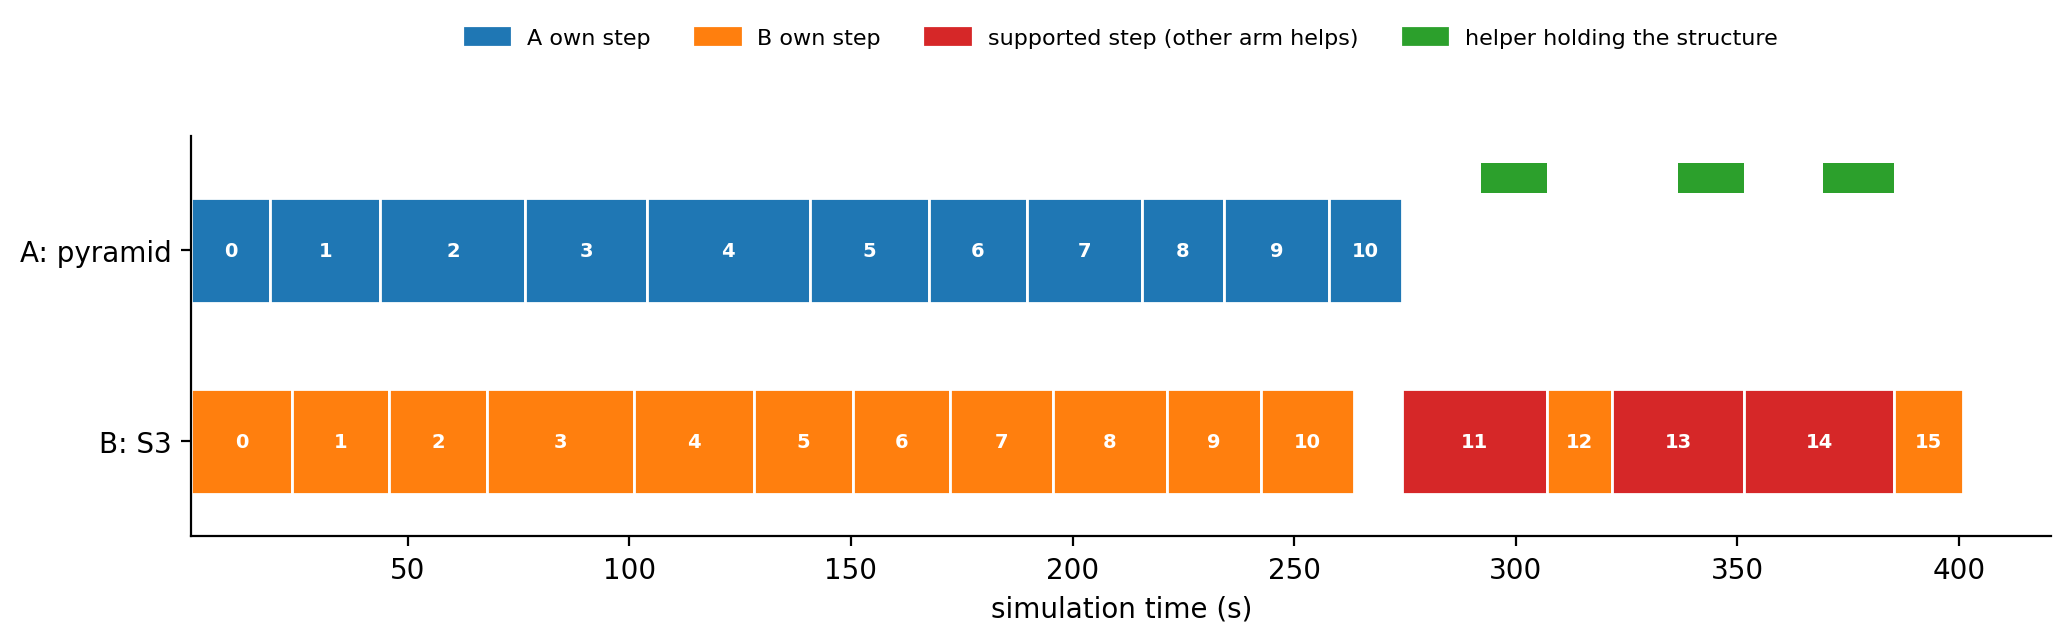
\includegraphics[width=\linewidth]{timeline_pyramid_s3.png}
\caption{Timeline of the pyramid + S3 run. The pyramid needs no support, so A builds
it alone and then helps B with S3's three supported steps.}
\end{figure}

% =====================================================================
\section{Towards real stud resistance (stud-fit mode)}\label{sec:studfit}

\keyidea{When every brick must be pushed onto the studs with real force, the
supported presses become the hard part. The latest run places all 27 bricks,
but several safety checks had to be loosened, and it still fails verification
on contacts.}

\subsection{What changes in this mode}
In the default cell a brick slides onto the studs under its own weight. With
\texttt{--stud-fit}, a brick that reaches the stud tops is held there until the
measured push reaches $n\times 8.9$\,N over its $n$ mating studs. The builder's
side grip slips at about 3\,N, so every brick is released on the stud tops and
pressed from above with the closed fingertips, ramping to 1.3$\times$ the needed
force. The pressing arm's joints are 5$\times$ stiffer during the press.

Supported steps needed the most work (Nov 10--16, about 40 commits and 27
diagnostic runs):
\begin{itemize}
\item \textbf{More and stronger supports.} The plan picks, among grips the force
      model rates safe, the one nearest the press, and forces a support wherever a
      brick or anything under it overhangs. S3 now has five supported steps (9, 11,
      13, 14, 15). The helper grips at about 43\,N per finger and holds at 20$\times$
      joint stiffness.
\item \textbf{Softer supported presses.} At 1.3$\times$ the needed force, S3's
      last brick broke the two-stud bridge joint below it, even though the
      force model rated that step safe with the support. Supported presses now
      ramp over 2\,s to 0.90$\times$ the needed force, and the brick is allowed
      through at 0.85$\times$.
\item \textbf{Joint breaker paused on supported steps.} Even then, the
      simulated joint load briefly crossed $u=1$ before push-through and spiked
      to $u=1.3$--$3.2$ at the moment the clutch welds took over. The break
      rule is now switched off from the start of a supported press until
      0.5\,s after the snap \emph{and} the helper has let go.
\item \textbf{Looser clearance limits near a holding helper.} A closed finger may
      overlap a placed brick's collision box by up to 1.25\,mm. The carried brick's
      corridor may overlap the helper by 1.5\,mm, and a supported pre-insert path
      may come within 2\,mm \emph{inside} the holding arm's spheres. Stud contacts
      may be 2.0\,mm deep (default 1.7\,mm), and a support may flex the structure
      by 1.5\,mm before it counts as ``displaced''. These limits apply only in
      stud-fit mode.
\end{itemize}

\subsection{Results}
\begin{figure}[H]
\centering
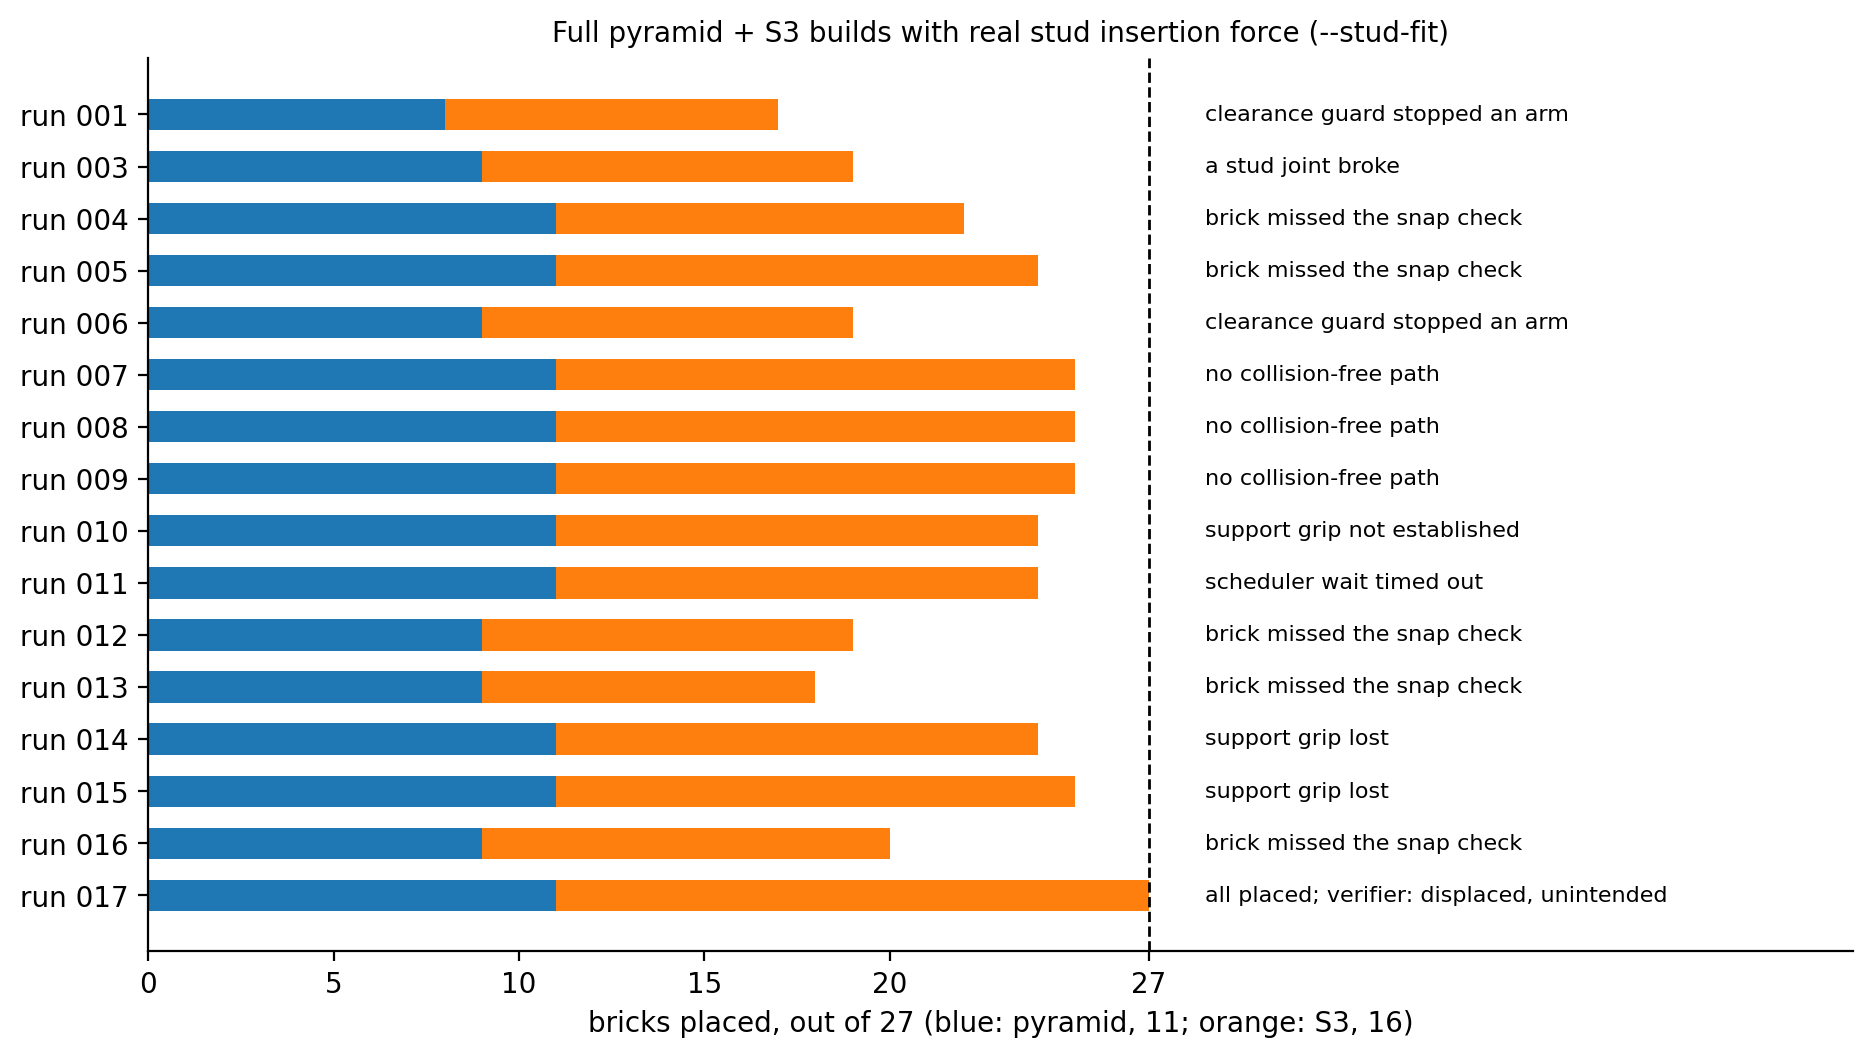
\includegraphics[width=\linewidth]{studfit_progress.png}
\caption{Every saved full pyramid + S3 stud-fit run and why it stopped. The
pyramid (blue) is reliably finished; the failures move later into S3 (orange)
as each cause is fixed.}
\label{fig:studfit}
\end{figure}

\begin{itemize}
\item \textbf{Run 017} is the first to place all 27 bricks against stud
      resistance (11/11 and 16/16, all five supports held). Every brick
      passed the snap check with at most 1.96\,mm sideways error, 0.33\,mm height
      error and 1.33$^\circ$ tilt. 219 motions were planned with no
      planning failure. The new recovery mattered: 14 support attempts were
      rejected and retried, 5 of them because only one finger made contact.
\item \textbf{It does not pass the verifier.} The audit recorded 5 unintended
      contacts and 23 ``displaced'' events:
      \begin{itemize}[nosep]
      \item 2 contacts were feeder bricks resting on the floor (0.01\,N). These are
            now exempt while an arm is staging.
      \item 3 contacts were the helper's finger brushing an S3 brick (0.9--2.1\,N)
            while it retracted.
      \item The 23 displacements moved four S3 bricks by up to 2.2\,mm during failed
            support attempts.
      \end{itemize}
      Its lowest measured clearance was $-0.86$\,mm, inside the loosened limits.
\item \textbf{The three newest commits target exactly these scrapes}
      (\S\ref{sec:recovery}): pull back further after a guard stop, then try a
      farther column. No full run with them has been saved yet.
\item \textbf{The previously open step now seats.} Diagnostic run 053 starts S3
      at step 13 with the earlier bricks pre-placed. It completes steps 13--15,
      and the verifier accepts it as a diagnostic, not as a full build.
\end{itemize}

\why{Pausing the joint breaker during supported presses deserves a plain
reading. The support is meant to carry the load around the weak joint. But the
simulated joints measure load only at the end of each frame, and they spike
when the welds hand over. So the breaker was reporting failures that a held
real structure would probably survive. The cost is that a supported step can no
longer \emph{fail} by breaking a joint in this mode. Until a full run passes the
verifier with the breaker active, or the breaker is made to ignore these
transient spikes, the stud-fit results are evidence of progress, not of
success.}

\section{Limitations and future work}\label{sec:limits}

\begin{itemize}
\item \textbf{Simulation only.} All results are from the Newton simulation; no
      physical robot was used.
\item \textbf{Ground-truth brick aim.} The brick-aim servo reads the brick's pose from
      the simulator. A camera-based estimator exists in the code base
      (\texttt{vision.py}, the FK aim mode) but the validated dual-arm runs do not use it.
\item \textbf{Clutch model.} In the default cell a brick seats under its own weight
      (0.6\,mm stud clearance) and the clutch is the snap check plus welds. With
      real stud resistance (\S\ref{sec:studfit}) all 27 bricks have been placed
      once, but no full run has passed the verifier yet. That mode also pauses the
      joint breaker during supported presses and loosens some clearance limits.
\item \textbf{Conservative stability model.} The LP ignores joint compliance, so a
      safety factor of 3 is used; for two of the four supports it cannot
      show a reduction in predicted load (\S\ref{sec:support}).
\item \textbf{Blueprint limits.} Silhouette carving cannot represent hidden
      cavities, and greedy tiling may bond complex shapes poorly.
\item \textbf{Sampled collision checks} are not a continuous-collision proof; the
      physics contact audit covers the gap in practice.
\end{itemize}
Natural next steps: a verified full stud-fit run with the newest recovery
code, a joint breaker that ignores weld hand-over spikes instead of being
paused, a fresh default-mode run on the current code, camera-based brick pose in
the dual-arm runs, a compliant joint model so the safety factor can drop, a support search that may grip the
critical pier joint from a second side, and transfer to the real cell.

\section{Conclusion}
The project turns a drawing or a brick list into two finished LEGO structures
built by two arms that share space safely and support each other. Every stage
uses an algorithm that can be explained in one sentence and checked with a
number: silhouette carving and greedy bonded tiling for the blueprint, a
layer-ordered plan with force-aware grips, a force-balance linear program for
support decisions, GPU motion planning with straight contact moves for control,
layered sphere-based collision checks with space reservations for two arms, and
a deterministic coordinator with a strict snap check and an independent
verifier for completion. The validated run meets all three of the supervisor's
requirements.

\appendix
\section{Reproducing the results}
From the repository root, with the shared environment \texttt{Sakib/.venv}:
\begin{verbatim}
# full build, about 30 min on one GPU; choose a new output folder
bash Kean/scripts/dual_build.sh --build-a arch --build-b S3 \
    --out Kean/results/my_run
Sakib/.venv/bin/python -m Kean.verify_dual --run Kean/results/my_run
bash Kean/scripts/play_run.sh --run Kean/results/my_run --port 8081 --loop

# this report's figures (CPU) and simulation stills (GPU)
Sakib/.venv/bin/python final_report/make_figures.py
Sakib/.venv/bin/python final_report/render_stills.py \
    Kean/results/dual_arch_s3_012 final_report/stills a:411:-0.25,0.16,0.06,-5,0
\end{verbatim}

\section{Glossary}
\begin{description}[leftmargin=3cm, style=nextline]
\item[Blueprint] The list of bricks (type, grid position, orientation) that makes the shape.
\item[Plan] The blueprint in build order, with grip, press point and support for each step.
\item[Visual hull] The largest shape consistent with all the silhouettes.
\item[Utilisation $u$] Load on a stud joint divided by its strength; $u\ge 1$ means it breaks.
\item[Support / helper] The other arm gripping the structure while a brick is pressed.
\item[cuRobo] NVIDIA's GPU motion planner for robot arms.
\item[IK] Inverse kinematics: joint angles that put the hand at a target.
\item[Reservation] Space an arm books before moving, so the other arm keeps out.
\item[Snap check] The test that decides a brick is in place (2\,mm, 1.5\,mm, 5$^\circ$, 5$^\circ$).
\item[Weld] The simulated stud clutch that holds a placed brick, and can break.
\end{description}

\end{document}
